% thesis_takada.tex
% ##################################################
\documentclass[a4paper,12pt]{article_vdlab_sotsuron}
\pagestyle{plain}

\usepackage{setspace}
\usepackage{graphicx}
\usepackage{amsmath,amssymb}
\usepackage{colortbl}
\usepackage{comment}
\usepackage{multirow}

\begin{document}
%文字間隔を設定
\kanjiskip = .0pt plus 3pt minus 3pt
\xkanjiskip = .0pt plus 3pt minus 3pt
\small
\setstretch{1.5}

% ##################################################
\begin{center}
  % 論文題目
  \jtitle{タイヤ-サスペンションHILSシステム\\における上下動再現手法の検討}
  \etitle{Study on Reproduction Method of Vertical Motion with\\Tire-Suspension Hardware-in-the-Loop Simulation System}
\end{center}

%目次の表示
\tableofcontents

% ##################################################
\newpage
\section{序論}
\subsection{タイヤとサスペンション}
自動車の基本的な機能である「走る」「曲がる」「止まる」といった運動は,すべて路面とタイヤとの間に発生する摩擦力によって実現している.そのため,タイヤは車両運動特性に大きな影響を与える重要な要素といえる.また,車体とタイヤはサスペンションによって連結されている.サスペンションは,車体重量を支持すると共に,車輪の上下振動を緩和,吸収して,振動が車体に直接伝達されることを防止する.また,路面間に発生する駆動力,制動力,横力など各種の路面反力を車体に伝達することで,車両運動性能に影響を与える.したがって,車両運動特性を把握するためには,タイヤとサスペンションを複合的に評価する必要がある.図~\ref{fig:tire_suspention}~にタイヤ-サスペンション機構を示す.

\vspace*{10mm}
\begin{figure}[h]
  \begin{center}
    \includegraphics[height=70mm]{figure/tire_suspension.eps}
    \vspace*{3mm}
    \caption{Tire-Suspension\cite{1}}
    \label{fig:tire_suspention}
  \end{center}
\end{figure}

% **************************************************
\newpage
\subsection{Hardware-in-the-Loop Simulation(HILS)システム}
車両運動性能を評価する手法として,シミュレーションや実車走行試験などが挙げられる.しかし,シミュレーションでは,評価対象のモデル化誤差が生じ,実車走行試験では,同一条件での試験が困難である.このような問題を解決するシステムとしてHILSシステムが用いられている\cite{2}.HILSとは,Hardware-in-the-Loop Simulationの略であり,評価対象のハードウェアをシミュレーションループ内に直接組み込み,対象のシステムの線形化や近似をすることなく評価を行うシステムである.このHILSシステムの主な利点として,以下の項目が挙げられる.

\begin{enumerate}
\item 開発期間の短縮が可能
\item 同一条件や様々な条件で繰り返し試験が可能
\item 評価対象のハードウェアを用いることでモデル化誤差が生じない
\item 実車試験で危険を伴う試験が可能
\end{enumerate}

\par
HILSシステムは,自動車業界の車両開発においても広く利用されている.
特にエンジンや変速機制御,ブレーキ制御等の開発,評価において開発期間の短縮や品質向上に寄与する重要なツールになりつつある\cite{3}.

\vspace*{10mm}
\begin{figure}[htp]
  \begin{center}
    \includegraphics[height=50mm]{figure/HILS_system.eps}
    \vspace*{3mm}
    \caption{HILS System\cite{4}}
    \label{fig:HILS_system}
  \end{center}
\end{figure}

% **************************************************
\newpage
\subsection{研究目的}
前述のように車両運動特性を評価するためにはタイヤとサスペンションの特性を複合的に評価する必要がある.これらを評価する手法として,シミュレーションや実車走行試験がある.シミュレーションによる評価では,タイヤやサスペンションは非線形特性を有するためモデル化することは困難である.一方,実車走行試験による評価では,路面状況や天候などの影響により測定値のばらつきが大きいことや同一条件で試験を行うことが困難である.\par
そこで本研究では,自動車のタイヤ-サスペンション系の上下動をHILSシステムを用いて評価する.タイヤ-サスペンション系をHILSシステムに組み込む場合,ハードウェア部の構成は,車体部を固定し,路面-車体間の相対変位をアクチュエートする1自由度系と,車体部を固定せず,路面と車体の変位をそれぞれアクチュエートする2自由度系が考えられる.2種類のハードウェア構成の概略図を図~\ref{fig:hardware_12}~に示す.ハードウェア部の構成がHILSの再現性に与える影響を評価するため,1自由度系と2自由度系の両方の構成が可能な試験装置を新たに開発し,これを用いてHILSシステムを構築した.両システムにおいて試験装置と解析モデルの差を比較することにより,上下動の再現性を評価した.

\vspace*{10mm}
\begin{figure}[h!]
  \begin{minipage}{0.5\hsize}
  \begin{center}
    \vspace*{10mm}
    \includegraphics[height=50mm]{figure/1dof_model.eps}
    \end{center}
    \begin{center}
    \vspace{3mm}
    \ (a)1DOF\
%     \label{fig:1dof_model} 
    \end{center}
  \end{minipage}
  \begin{minipage}{0.5\hsize}
     \begin{center}
      \includegraphics[height=60mm]{figure/2dof_model.eps}
      \end{center}
      \begin{center}
      \vspace{3mm}
      \ (b)2DOF\
%       \label{fig:2dof_model}
    \end{center}
  \end{minipage}
  \vspace*{3mm}
  \caption{Hardware}
    \label{fig:hardware_12}
 \end{figure}

% #################################################
\newpage
\section{試験装置の開発}
\subsection{装置の構成}
本研究で開発した試験装置を図~\ref{fig:test_machine}~に示す.本試験装置はタイヤ-サスペンション系を模擬してあり,主に路面部・タイヤ部・車体部・外枠フレームから構成される.上下に可動する部分にはリニアベアリングを取り付けた.路面部と車体部にはそれぞれアクチュエータを取り付けた.路面部はスライダ-クランク機構により,車体部はボールねじ機構により上下方向に加振できる.タイヤ部と車体部は実際の車両に近づけるため,重量比や弾性係数,減衰係数を調整した.車体部を外枠フレームに対して固定し,アクチュエータを切ることで1自由度系を再現できる.部品は主にミスミのアルミフレームを使用した.メリットとして,組み立てや交換が容易であることや,コストの低さ,入手時間の短さなどが挙げられる.\par

\vspace*{10mm}
\begin{figure}[htp]
  \begin{center}
    \includegraphics[height=100mm]{figure/test_machine.eps}
    \vspace*{3mm}
    \caption{Tire-Suspension Testing Machine}
    \label{fig:test_machine}
  \end{center}
\end{figure}

% **************************************************
\newpage
\subsection{路面部の設計}
路面部を図~\ref{fig:b1_gf}~に示す.アクチュエータとしてECモータを取り付け,スライダ-クランク機構によって上下方向へ加振する.モータには回転軸を取り付けた.回転軸の両端を,ベアリングホルダを用いて支えることで,モータへかかる負荷が軽減でき,壊れにくくなる.また,路面部とモータの間にばねを取り付けた。ばねが可動部の荷重を支えるため、モータへかかる負荷を軽減でき、可動部を動かすためのトルクのみで良いことになる.

\vspace*{10mm}
\begin{figure}[h!]
  \begin{minipage}{0.5\hsize}
  \begin{center} 
    \includegraphics[height=40mm]{figure/b1_gf_front.eps}
    \end{center}
    \begin{center}
    \vspace{3mm}
    \ (a)Front\
%     \label{fig:b1_gf_front} 
    \end{center}
  \end{minipage}
  \begin{minipage}{0.5\hsize}
     \begin{center}
      \includegraphics[height=40mm]{figure/b1_gf_right.eps}
      \end{center}
      \begin{center}
      \vspace{3mm}
      \ (b)Right\
%       \label{fig:b1_gf_right}
    \end{center}
  \end{minipage}
  \vspace*{3mm}
  \caption{Road}
    \label{fig:b1_gf}
 \end{figure}

% --------------------------------------------------
\newpage
\subsubsection{スライダ-クランク機構の選定}
スライダ-クランク機構は回転運動を直動運動へ変換する機構のひとつであり,図~\ref{fig:slider_crank}~に示すように回転するクランクとコネクティングロッドから構成される.本研究では路面の変位を±30mm確保するためにクランク長rは45mmを選定した.この場合,クランクの回転角$θ_A$が45deg回転するとコネクティングロッドの先端は$45/\sqrt{2}=31.2$mm変位し,スライダ-クランクが特異姿勢に入らない範囲内で使用できる.\par
コネクティングロッドの先端に力Fが加わったときに,モータへかかるトルクTは以下の式で表される.

\begin{eqnarray}
 \label{eq:slider_crank} T &=& rF\cos\theta_B\cos\theta_A 
\end{eqnarray}

F=80Nの際のモータへかかる負荷は図~\ref{fig:slider_crank_torque}~のようになる.今回はコネクティングロッドの長さlは90mmを選定した.

\vspace*{10mm}
\begin{figure}[htp]
  \begin{center}
    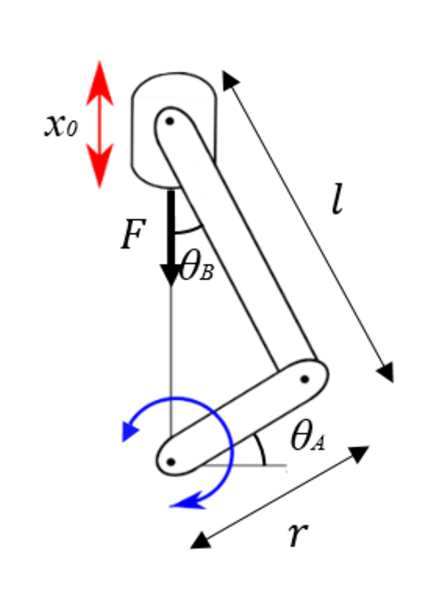
\includegraphics[height=50mm]{figure/slider_crank.eps}
    \vspace*{3mm}
    \caption{Slider Crank Mechanism}
    \label{fig:slider_crank}
  \end{center}
\end{figure}

\vspace*{10mm}
\begin{figure}[htp]
  \hspace*{50mm}
    \includegraphics[scale=1]{figure/slider_crank_torque.eps}
    \vspace*{3mm}
    \caption{Torque Transmissibility}
    \label{fig:slider_crank_torque}
\end{figure}

% --------------------------------------------------
\newpage
\subsubsection{路面部モータの選定}
路面部のアクチュエータとして,図~\ref{fig:ecmax40}~に示すmaxon japan株式会社のECブラシレスモータ「EC max40 283867」を選定した.モータスペックは表~\ref{tab:ecmax40}~の通りである.モータの先端にはギアヘッドが取り付けられ,回転方向や角度を検出する電子部品としてエンコーダが取り付けられている.このモータにはmaxon japan株式会社のプラネタリギアヘッド「GP42C 203126」とエンコーダ「HEDL5540 110516」を取り付けた.そでぞれの仕様を表~\ref{tab:113:1}~,表~\ref{tab:500pulse}~に示す.

\vspace*{10mm}
\begin{figure}[htp]
  \begin{minipage}{0.4\textwidth}
    \begin{center}
      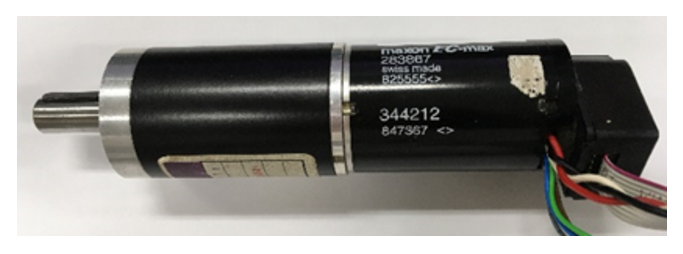
\includegraphics[height=20mm]{figure/ecmax40.eps}
      \vspace*{3mm}
      \caption{ECmax40 283867}
      \label{fig:ecmax40}
    \end{center}
  \end{minipage}
  \begin{minipage}{0.6\textwidth}
      \begin{center}
	\makeatletter
	\def\@captype{table}   
	\makeatother
	\caption{Specification of EC Servomotor(283867)}
	\label{tab:ecmax40}
	  \begin{tabular}{cc}\hline
	    Nominal output & 70 [W] \\
	    Nominal voltage & 24 [V] \\
	    Nominal speed & 12000 [rpm] \\
	    Max continuous Torque & 89.6 [mNm] \\
	    Max continuous current & 3.44 [A] \\
	    Torque constant & 28 [mNm/A] \\
	    Speed constant & 341 [rpm/V] \\\hline 
	  \end{tabular}  
	\end{center}
  \end{minipage}
\end{figure}

\vspace*{10mm}
\begin{table}[htp]
  \begin{minipage}{0.5\textwidth}
    \begin{center}
      \makeatletter
	\def\@captype{table}   
	\makeatother
	\caption{Specification Gearhead(203126)}
	\label{tab:113:1}
	  \begin{tabular}{cc}\hline
	    Gear Ratio & 113:1 \\
	    Rated speed & 8000 [rpm] \\
	    Backlash & 1.0 [deg] \\
	    Max continuous torque & 15 [Nm] \\\hline
	  \end{tabular}  
    \end{center}
  \end{minipage}
  \begin{minipage}{0.5\textwidth}
      \begin{center}
	\makeatletter
	\def\@captype{table}   
	\makeatother
	\caption{Specification of Encoder(110516)}
	\label{tab:500pulse}
	  \begin{tabular}{cc}\hline
	    Encoder Resolution & 500 [count/rev] \\
	    Max frequency & 100 [kHz] \\ 
	    Allowable maximum speed & 12000 [rpm] \\\hline
	  \end{tabular}  
	\end{center}
  \end{minipage}
\end{table}

\vspace*{10mm}
このモータに先述したスライダ-クランク機構を取り付けた場合、エンコーダ1pulseあたりの変位xは、パルス数をpとして式~\ref{eq:mm_to_deg}~で表される。しかし今回は簡易的に式~\ref{eq:mm_to_pulse}~から算出した。モータの回転角と変位の関係を表したグラフを図~\ref{fig:mm_to_pulse}~に示す。

\begin{eqnarray}
 \label{eq:mm_to_deg} x &=& 45(1-\cos \frac{2\pi p}{500\cdot 113})+\frac{45^2}{4\cdot 90} (1+\cos 2 \frac{2\pi p}{500\cdot 113}) \\
 \label{eq:mm_to_pulse} x &=& 45sin\frac{2\pi p}{500\cdot 113}
\end{eqnarray}

\newpage
\begin{figure}[htp]
  \hspace*{45mm}
    \includegraphics[scale=1]{figure/mm_to_pulse.eps}
    \vspace*{3mm}
    \caption{Displacement Pulse}
    \label{fig:mm_to_pulse}
\end{figure}

\vspace*{10mm}
このモータに対して加速度一定のスイープ波を入力し,周波数応答を確認した.ボード線図を図~\ref{fig:ecmax40_sweep}~に示す.ゲインがフラットであることから,モータの周波数依存性は殆ど無いと言える.

\vspace*{10mm}
\begin{figure}[h!]
  \begin{tabular}{cc}
  \begin{minipage}{0.5\hsize}
  \begin{center} 
    \includegraphics[scale=1]{figure/ecmax40_sweep_input.eps}
    \end{center}
    \begin{center}
    \vspace{3mm}
    \ (a)Input\
%     \label{fig:ecmax40_sweep_input} 
    \end{center}
  \end{minipage}
  \begin{minipage}{0.5\hsize}
     \begin{center} 
      \includegraphics[scale=1]{figure/ecmax40_sweep.eps}
    \end{center}
      \vspace*{-20mm}
    \begin{center}
      \ Input:Road Input\\
      \ Output:Encorder\\
      \vspace*{3mm}
      \ (b)Boad Diagram\\
%       \label{fig:ecmax40_sweep}
    \end{center}
  \end{minipage}
  \end{tabular}
  \vspace*{3mm}
  \caption{Frequency Responce(283867)}
    \label{fig:ecmax40_sweep}
\end{figure}

\vspace*{10mm}
また,モータスペックから,本研究で用いるスライダ-クランク機構の変位限界,速度限界,加速度限界が求められる.rをクランク長,Nを最大許容回転数,Tを最大連続トルク,mを可動部質量とし,変位限界,速度限界,加速度限界は以下の式から算出できる.

\newpage
\begin{eqnarray}
 \label{eq:ecmax40_x} X_{limit} &=& 2r \\
 \label{eq:ecmax40_v} V_{limit} &=& lN \\
 \label{eq:ecmax40_a} A_{limit} &=& 2\pi\frac{T}{ml}
\end{eqnarray}

\vspace*{10mm}
ここで,lはモータ1回転当たりの変位であり,ギア比iを用いて以下の式から簡易的に算出した.

\begin{eqnarray}
 \label{eq:l} l = \frac{2r}{\pi\cdot i/2\pi} = 4r/i
\end{eqnarray}

\vspace*{10mm}
式~\ref{eq:ecmax40_x}~,~\ref{eq:ecmax40_v}~,~\ref{eq:ecmax40_a}~を用いて,各限界における周波数fと変位Aの関係を以下に示す.

\begin{eqnarray}
 \label{eq:ecmax40_xx} &&A_{X_{limit}} = X_{limit} = 2r \\
 \label{eq:ecmax40_vx} &&A_{V_{limit}} = V_{limit}\frac{1}{2\pi f} =  lN\frac{1}{2\pi f}\\
 \label{eq:ecmax40_ax} &&A_{A_{limit}} = A_{limit}\frac{1}{(2\pi f)^2} = 2\pi\frac{T}{ml}\frac{1}{(2\pi f)^2}
\end{eqnarray}

\vspace*{10mm}
これらを用いて,横軸を周波数,縦軸を変位とした対数グラフに各限界の式をプロットしたものを性能線図と呼ぶ.クランク長rを45mm,可動部質量mを8kgとしたときの性能線図を図~\ref{fig:seinou}~に示す.

\vspace*{10mm}
\begin{figure}[htp]
  \hspace*{45mm}
    \includegraphics[scale=1]{figure/seinou.eps}
    \vspace*{3mm}
    \caption{Performance Diagram(283867)}
    \label{fig:seinou}
\end{figure}

% --------------------------------------------------
\newpage
\subsubsection{路面部ばねの選定}
路面部のばねは図~\ref{fig:11-2527}~に示すサミニの「11-2527」を選定した.使用を表~\ref{tab:11-2527}~に示す.

\vspace*{10mm}
\begin{figure}[htp]
  \begin{minipage}{0.5\textwidth}
    \begin{center}
      \includegraphics[height=60mm]{figure/11-2527.eps}
      \vspace*{3mm}
      \caption{Spring 11-2527}
      \label{fig:11-2527}
    \end{center}
  \end{minipage}
  \begin{minipage}{0.5\textwidth}
      \begin{center}
	\makeatletter
	\def\@captype{table}   
	\makeatother
	\caption{Specification of Spring(11-2527)\cite{5}}
	\label{tab:11-2527}
	  \begin{tabular}{cc}\hline
	    Material & SWP-A \\
	    Wire Diameter & 2 [mm] \\
	    Outer Diameter & 25 [mm] \\
	    Number of Active Coils & 14.75 [-] \\
	    Free Length & 150 [mm] \\
	    Spring constant & 0.88 [N/mm] \\\hline
	  \end{tabular}  
	\end{center}
  \end{minipage}
\end{figure}

% --------------------------------------------------
\vspace*{10mm}
\subsubsection{リニアベアリングの選定}
選定したリニアベアリングを図~\ref{fig:liner_bearing}~に示す.シャフトに沿ってリニアベアリングが直動することにより,可動部が上下に直動できる.可動部を挟み込むようにリニアベアリングを配置することで,こじりが生じにくい.タイヤ部と車体部にも同様のリニアベアリングを使用した.

\vspace*{10mm}
\begin{figure}[htp]
  \begin{center}
    \includegraphics[height=60mm]{figure/liner_bearing.eps}
    \vspace*{3mm}
    \caption{Linear Bearnig}
    \label{fig:liner_bearing}
  \end{center}
\end{figure}

% **************************************************
\newpage
\subsection{タイヤ部の設計}
タイヤ部を図~\ref{fig:1f}~に示す.アルミフレームをI字状に配置し,その両端にリニアベアリングを取り付けた.

\vspace*{10mm}
\begin{figure}[htp]
  \begin{center}
    \includegraphics[height=50mm]{figure/1f.eps}
    \vspace*{3mm}
    \caption{Tire}
    \label{fig:1f}
  \end{center}
\end{figure}

% --------------------------------------------------
\vspace*{10mm}
\subsubsection{タイヤ部ばねの選定}
タイヤ部のばねは図~\ref{fig:11-2526}~に示すサミニの「11-2526」を選定した.性能表を表~\ref{tab:11-2526}~に示す.

\vspace*{10mm}
\begin{figure}[htp]
  \begin{minipage}{0.5\textwidth}
    \begin{center}
      \includegraphics[height=60mm]{figure/11-2526.eps}
      \vspace*{3mm}
      \caption{Spring 11-2526}
      \label{fig:11-2526}
    \end{center}
  \end{minipage}
  \begin{minipage}{0.5\textwidth}
      \begin{center}
	\makeatletter
	\def\@captype{table}   
	\makeatother
	\caption{Specification of Spring(11-2526)\cite{5}}
	\label{tab:11-2526}
	  \begin{tabular}{cc}\hline
	    Material & SWP-A \\
	    Wire Diameter & 2 [mm] \\
	    Outer Diameter & 25 [mm] \\
	    Number of Active Coils & 11.73 [-] \\
	    Free Length & 120 [mm] \\
	    Spring constant & 1.1 [N/mm] \\\hline
	  \end{tabular}  
	\end{center}
  \end{minipage}
\end{figure}

% **************************************************
\newpage
\subsection{車体部の設計}
車体部を図~\ref{fig:2f}~に示す.車体部は主にアルミフレームで構成され,大きくリニアブッシュとダンパ・ロードセルを取り付ける中央部と,ばねの取り付けとダンパがストローク限界を超えないためのストッパになる下部と,ボールねじを取り付ける上部に分けられる.ダンパのためのストッパには衝撃を吸収するウレタンシートを貼った.上部にあるボールねじを取り付けるプレートは,上方向への曲げ強度を上げるためにコの字型のものを使用した.ボールねじ付きECモータはアルミフレームを用いて外枠フレームに固定した.

\vspace*{10mm}
\begin{figure}[h!]
  \begin{tabular}{cc}
  \begin{minipage}{0.5\hsize}
  \begin{center} 
    \includegraphics[height=80mm]{figure/2f_front.eps}
    \end{center}
    \begin{center}
    \vspace{3mm}
    \ (a)Front\
%     \label{fig:2f_front} 
    \end{center}
  \end{minipage}
  \begin{minipage}{0.5\hsize}
     \begin{center}
      \includegraphics[height=80mm]{figure/2f_right.eps}
      \end{center}
      \begin{center}
      \vspace{3mm}
      \ (b)Right\
%       \label{fig:2f_right}
    \end{center}
  \end{minipage}
  \end{tabular}
  \vspace*{3mm}
  \caption{Body}
    \label{fig:2f}
 \end{figure}

% --------------------------------------------------
\newpage
\subsubsection{車体部ばねの選定}
車体部のばねを図~\ref{fig:iida}~に,性能表を表~\ref{tab:iida}~に示す.このばねは線径,外径が大きく,市販のばねで条件を満たすものがなかったため,有限会社 飯田スプリングにて特注で製作して頂いた.このばねの詳しい要目表は付録を参照してほしい.

\vspace*{10mm}
\begin{figure}[htp]
  \begin{minipage}{0.5\textwidth}
    \begin{center}
      \includegraphics[height=60mm]{figure/iida.eps}
      \vspace*{3mm}
      \caption{Order Spring}
      \label{fig:iida}
    \end{center}
  \end{minipage}
  \begin{minipage}{0.5\textwidth}
      \begin{center}
	\makeatletter
	\def\@captype{table}   
	\makeatother
	\caption{Specification of Order Spring}
	\label{tab:iida}
	  \begin{tabular}{cc}\hline
	    Material & SWP-B \\
	    Wire Diameter & 5.5 [mm] \\
	    Outer Diameter & 130 [mm] \\
	    Number of Active Coils & 11.5 [-] \\
	    Free Length & 270 [mm] \\
	    Spring constant & 0.405 [N/mm] \\\hline
	  \end{tabular}  
	\end{center}
  \end{minipage}
\end{figure}

% --------------------------------------------------
\vspace*{10mm}
\subsubsection{ダンパの選定}
ダンパは図~\ref{fig:2ks95}~に示すAirpot社のエアダンパ「2KS95」を選定した.性能表を表~\ref{tab:2ks95}~に示す.このエアダンパにはダンピング調節ねじがあり,ねじの回転量に応じて減衰力を変更することができる.

\vspace*{10mm}
\begin{figure}[htp]
  \begin{minipage}{0.5\textwidth}
    \begin{center}
      \includegraphics[height=60mm]{figure/2ks95.eps}
      \vspace*{3mm}
      \caption{Airpot 2KS95}
      \label{fig:2ks95}
    \end{center}
  \end{minipage}
  \begin{minipage}{0.5\textwidth}
      \begin{center}
	\makeatletter
	\def\@captype{table}   
	\makeatother
	\caption{Specification of Air Damper}
	\label{tab:2ks95}
	  \begin{tabular}{cc}\hline
	    Diameter of Cylinder & 111 [mm] \\
	    Damping Coefficient & 5.5 [N/mm/s] \\
	    Maximum Tensile Force & 130 [N] \\
	    Maximum Compression Force & 11.5 [N] \\
	    Maximum Stroke & 50.2 [mm] \\\hline
	  \end{tabular}  
	\end{center}
  \end{minipage}
\end{figure}

\newpage
エアダンパが許容するストロークを超えて伸びたり縮んだりすると,破損の原因となる.そこでエアダンパが許容ストロークを超えないようにストッパを取り付けた.表~\ref{tab:2ks95}~から分かるようにストロークは50.2mmであるため,ピストンが中心位置にある状態から±20mmの位置にストッパを取り付け、引張・圧縮ともに5.2mmのクリアランスを確保した.図~\ref{fig:damp_stop}~にストッパに当たる様子を、図~\ref{fig:damp_stop_cad}~にストッパのレイアウトを示す.

\vspace*{10mm}
\begin{figure}[h!]
  \begin{tabular}{cc}
  \begin{minipage}{0.5\hsize}
  \begin{center} 
    \includegraphics[height=70mm]{figure/damp_min.eps}
    \end{center}
    \begin{center}
    \vspace{3mm}
    \ (a)Minimum Stroke\
%     \label{fig:damp_min} 
    \end{center}
  \end{minipage}
  \begin{minipage}{0.5\hsize}
     \begin{center}
      \includegraphics[height=70mm]{figure/damp_max.eps}
      \end{center}
      \begin{center}
      \vspace{3mm}
      \ (b)Maximum Stroke\
%       \label{fig:damp_max}
    \end{center}
  \end{minipage}
  \end{tabular}
  \vspace*{3mm}
  \caption{Stopper of Damper}
    \label{fig:damp_stop}
\end{figure}
 
\vspace*{10mm}
\begin{figure}[h!]
  \begin{tabular}{cc}
  \begin{minipage}{0.5\hsize}
  \begin{center} 
    \includegraphics[height=50mm]{figure/damp_min_cad.eps}
    \end{center}
    \begin{center}
    \vspace{3mm}
    \ (a)Minimum Stroke\
%     \label{fig:damp_min_cad} 
    \end{center}
  \end{minipage}
  \begin{minipage}{0.5\hsize}
     \begin{center}
      \includegraphics[height=50mm]{figure/damp_max_cad.eps}
      \end{center}
      \begin{center}
      \vspace{3mm}
      \ (b)Maximum Stroke\
%       \label{fig:damp_max_cad}
    \end{center}
  \end{minipage}
  \end{tabular}
  \vspace*{3mm}
  \caption{Layout of Damper Stopper}
    \label{fig:damp_stop_cad}
\end{figure}

% --------------------------------------------------
\newpage
\subsubsection{車体部モータの選定}
車体部のアクチュエータとして,図~\ref{fig:ec22}~に示すmaxon japan株式会社のECブラシレスモータ「EC22 386658」を選定した.モータスペックは表~\ref{tab:ec22}~の通りである.モータの先端にはボールねじ付きのギアヘッドが取り付けられ,回転方向や角度を検出する電子部品としてエンコーダが取り付けられている.このモータにはmaxon japan株式会社のスピンドルドライブ「GP22S 363863」とエンコーダ「エンコーダMR 201937」を取り付けてある.それぞれの仕様を表~\ref{tab:spindle}~,表~\ref{tab:512pulse}~に示す.

\vspace*{10mm}
\begin{figure}[htp]
  \begin{minipage}{0.3\textwidth}
    \begin{center}
      \includegraphics[height=40mm]{figure/ec22.eps}
      \vspace*{3mm}
      \caption{EC22 386658}
      \label{fig:ec22}
    \end{center}
  \end{minipage}
  \begin{minipage}{0.7\textwidth}
      \begin{center}
	\makeatletter
	\def\@captype{table}   
	\makeatother
	\caption{Specification of EC Servomotor(386658)}
	\label{tab:ec22}
	  \begin{tabular}{cc}\hline
	    Nominal output & 40 [W] \\
	    Nominal voltage & 24 [V] \\
	    Nominal speed & 35200 [rpm] \\
	    Max continuous Torque & 20.7 [mNm] \\
	    Max continuous current & 3.29 [A] \\
	    Torque constant & 6.49 [mNm/A] \\
	    Speed constant & 1470 [rpm/V] \\\hline 
	  \end{tabular}  
	\end{center}
  \end{minipage}
\end{figure}

\vspace*{10mm}
\begin{table}[htp]
  \begin{center}
    \makeatletter
      \def\@captype{table}   
      \makeatother
      \caption{Specification of Spindle Drive(363863)}
      \label{tab:spindle}
	\begin{tabular}{cc}\hline
	  Gear Ratio & 1:1 \\
	  Rated speed & 8000 [rpm] \\
	  Lead & 2.0 [mm] \\
	  Spindle Length & 151 [mm] \\\hline
	\end{tabular}  
  \end{center}
\end{table}

\vspace*{10mm}
\begin{table}[htp]
    \begin{center}
      \makeatletter
      \def\@captype{table}   
      \makeatother
      \caption{Specification of Encoder(201937)}
      \label{tab:512pulse}
	\begin{tabular}{cc}\hline
	  Encoder Resolution & 512 [count/rev] \\
	  Max frequency & 320 [kHz] \\ 
	  Allowable maximum speed & 37500 [rpm] \\\hline
	\end{tabular}  
      \end{center}
\end{table}

\newpage
このモータに対して変位一定のスイープ波を入力し,周波数応答を確認した.ボード線図を図~\ref{fig:ec22_sweep}~に示す.ゲインがフラットであることから,モータの周波数依存性は殆ど無いと言える.
 
\vspace*{10mm}
\begin{figure}[h!]
  \begin{tabular}{cc}
  \begin{minipage}{0.5\hsize}
  \begin{center} 
    \includegraphics[scale=1]{figure/ec22_sweep_input.eps}
    \end{center}
    \begin{center}
    \vspace{3mm}
    \ (a)Input\
%     \label{fig:ec22_sweep_input} 
    \end{center}
  \end{minipage}
  \begin{minipage}{0.5\hsize}
     \begin{center} 
      \vspace*{10mm}
      \includegraphics[scale=1]{figure/ec22_sweep.eps}
    \end{center}
    \begin{center}
      \ Input:Road Input\\
      \ Output:Encorder\\
      \vspace*{3mm}
      \ (b)Boad Diagram\\
%       \label{fig:ec22_sweep}
    \end{center}
  \end{minipage}
  \end{tabular}
  \vspace*{3mm}
  \caption{Frequency Responce(386658)}
    \label{fig:ec22_sweep}
\end{figure}

\newpage
なお,同じくこのモータに対して加速度一定のスイープ派を入力した場合のボード線図を図~\ref{fig:ec22_sweep_bat}~に示す.図~\ref{fig:ec22_sweep_bat}~(b)から,3Hz程度から位相が遅れていくことがわかる.これはモータ1回展あたりの分解能より小さい入力を与えたためであると考えられる。モータの一回転あたりの分解能が2/(512$\times$4)=0.001mmである。一方、入力はシリアル通信を用い、通信周期は2msで行った。図~\ref{fig:ec22_sweep_bat}~(a)から,200sから入力が周波数3Hz以上、振幅0.3mm以下になることがわかり、通信は1ステップあたり0.3/3/(1/0.002)=0.0002mmの変位を送る。これより、入力がモータの分解能よりも小さくなってしまったことがわかる。ただし、この検証は未実施である。

\vspace*{10mm}
\begin{figure}[h!]
  \begin{tabular}{cc}
  \begin{minipage}{0.5\hsize}
  \begin{center} 
    \includegraphics[scale=1]{figure/ec22_sweep_input_bat.eps}
    \end{center}
    \begin{center}
    \vspace{3mm}
    \ (a)Input\
%     \label{fig:ec22_sweep_input_bat} 
    \end{center}
  \end{minipage}
  \begin{minipage}{0.5\hsize}
     \begin{center} 
      \includegraphics[scale=1]{figure/ec22_sweep_bat.eps}
    \end{center}
    \begin{center}
      \ Input:Road Input\\
      \ Output:Encorder\\
      \vspace*{3mm}
      \ (b)Boad Diagram\\
%       \label{fig:ec22_sweep_bat}
    \end{center}
  \end{minipage}
  \end{tabular}
  \vspace*{3mm}
  \caption{BAD Frequency Responce(386658)}
    \label{fig:ec22_sweep_bat}
\end{figure}

\newpage
路面部モータの時と同様に,モータスペックから変位限界,速度限界,加速度限界が以下のように求められる.

\begin{eqnarray}
 \label{eq:ec22_x} &&A_{X_{limit}} = 0.03 [m] \\
 \label{eq:ec22_v} &&A_{V_{limit}} = lN\frac{1}{2\pi f} = 187/f [m/s]\\
 \label{eq:ec22_a} &&A_{A_{limit}} = 2\pi\frac{T}{ml}\frac{1}{(2\pi f)^2} = 0.26/f^2 [m/s^2]
\end{eqnarray}

\vspace*{10mm}
ここで,可動部質量mは6.4kgであり,変位限界はモータのストッパから決定した.モータのストッパは,ボールねじが可動部から抜けることや,先端がロードセルとぶつかることを防ぐ役割を果たし,外枠フレームに取り付けた.図~\ref{fig:seinou_2f}~に性能線図を示す.

\vspace*{10mm}
\begin{figure}[htp]
  \hspace*{45mm}
    \includegraphics[scale=1]{figure/seinou_2f.eps}
    \vspace*{3mm}
    \caption{Paformance Diagram(386658)}
    \label{fig:seinou_2f}
\end{figure}

% **************************************************
\newpage
\subsection{外枠フレームの設計}
外枠フレームを図~\ref{fig:frame}~に示す.外枠フレームには車体部のモータとレーザ変位計を取り付けるアルミフレームと,モータのストッパの役割をするアルミフレームが取り付けられている.ストッパは車体部がセット位置から上下に30mm可動できる位置に取り付けた.ストッパのアルミフレームを用いて車体部を挟み込むことで,ばね上固定の1自由度系を再現できる.図~\ref{fig:motor_stop}~に車体部がストッパに当たる様子を示す.

\vspace*{10mm}
\begin{figure}[htp]
  \begin{center}
    \includegraphics[height=70mm]{figure/frame.eps}
    \vspace*{3mm}
    \caption{Frame}
    \label{fig:frame}
  \end{center}
\end{figure}

\vspace*{10mm}
\begin{figure}[h!]
  \begin{tabular}{cc}
  \begin{minipage}{0.5\hsize}
  \begin{center} 
    \includegraphics[height=60mm]{figure/motor_min.eps}
    \end{center}
    \begin{center}
    \vspace{3mm}
    \ (a)Minimum Stroke\
%     \label{fig:motor_min} 
    \end{center}
  \end{minipage}
  \begin{minipage}{0.5\hsize}
     \begin{center}
      \includegraphics[height=60mm]{figure/motor_max.eps}
      \end{center}
      \begin{center}
      \vspace{3mm}
      \ (b)Maximum Stroke\
%       \label{fig:motor_max}
    \end{center}
  \end{minipage}
  \end{tabular}
  \vspace*{3mm}
  \caption{Stopper of Motor}
    \label{fig:motor_stop}
 \end{figure}

% **************************************************
\newpage
\subsection{設計時のトラブル}
設計当初,試験装置に用いるばねは表~\ref{tab:buckled_spring}~に示す3種類を予定していた.しかし,試験装置の重量が予定していた重量の2倍以上になったことなどにより,組み立てた際に座屈してしまった.ばねは自然長と外径の比が0.8~4.0が望ましいとされ,過大の場合は座屈や偏心を生じ,過小の場合はたわみ量が少ないばねということになり,計算値通りのばね定数を得られないことがある\cite{5}.ばねが座屈した様子を図~\ref{fig:buckled_spring}~に示す.

\vspace*{10mm}
\begin{table}[htp]
    \begin{center}
      \makeatletter
      \def\@captype{table}   
      \makeatother
      \caption{Initial Spring Design}
	\label{tab:buckled_spring}
	  \begin{tabular}{cccc}\hline
	    Parameter & Road & Tire & Body \\\hline
	    Material[-] & SUS304WPB & SUS304WPB & SUS304WPB \\
	    Wire Diameter[mm] & 1.6 & 1.6 & 1.2 \\
	    Outer Diameter[mm] & 17.6 & 16 & 16 \\
	    Number of Active Coils[-] & 18.5 & 23 & 23.75 \\
	    Free Length[mm] & 165 & 150 & 150 \\
	    Spring constant[N/mm] & 0.741 & 0.820 & 0.405 \\\hline
	\end{tabular}
      \end{center}
\end{table}

\vspace*{10mm}
\begin{figure}[htp]
  \begin{center}
    \includegraphics[height=70mm]{figure/buckled_spring.eps}
    \vspace*{3mm}
    \caption{Buckled Spring}
    \label{fig:buckled_spring}
  \end{center}
\end{figure}

% **************************************************
\newpage
\subsection{試験装置の組立}
図~\ref{fig:testing_machine}~に組み立てた試験装置を示す.また,表~\ref{tab:testing_machine}~に装置の諸元を示す.装置の組立は路面部のスライダ-クランク機構から行った.外枠フレームに対して回転軸が中心になるように計りながら路面部を組み立てた.その後,タイヤ部,車体部の順に組み立て,最後に2つのモータを取り付けた.モータを最後に取り付けることで,組立時にモータへ無理な負荷をかけてしまうリスクが低減できる.

\vspace*{10mm}
\begin{figure}[htp]
  \begin{center}
    \includegraphics[height=80mm]{figure/testing_machine.eps}
    \vspace*{3mm}
    \caption{Testing Machine}
    \label{fig:testing_machine}
  \end{center}
\end{figure}

\vspace*{10mm}
\begin{table}[htp]
    \begin{center}
      \makeatletter
      \def\@captype{table}   
      \makeatother
      \caption{Specification of Testing Machine}
	\label{tab:testing_machine}
	  \begin{tabular}{cc}\hline
	    Oveall Height [mm] & 860\\
	    Overall Length [mm] & 460\\ 
	    Overall Width [mm] & 400\\
	    Sprung Mass $m_2$ [kg] & 6.4 \\
	    Unsprung Mass $m_1$ [kg] & 1.2\\ 
	    Spring constant $k_2$ [N/m] & 405\\
	    Spring constant $k_1$ [N/m] & 2200\\\hline
	\end{tabular}  
      \end{center}
\end{table}

% #################################################
\newpage
\section{タイヤ-サスペンションHILSシステム}
\subsection{システムの概要}
本研究で新たに構築したタイヤ-サスペンションHILSシステムの概要を図~\ref{fig:HILS}~に示す.タイヤ-サスペンションHILSシステムは,ハードウェア部である前章で示した試験装置と,ソフトウェア部である車両運動解析やシステム制御を行うPCから構成される.本システムでは試験装置から計測されたダンパ力を用いてリアルタイム車両運動解析を実行し,ばね上-ばね下間相対変位を算出する.この解析結果の基づきアクチュエータを制御することでリアルタイムに車両の上下動を再現している.ここで,ばね上とは前章の車体部,ばね下はタイヤ部を指し,以降この表現を用いることとする.

\vspace*{10mm}
\begin{figure}[htp]
  \begin{center}
    \includegraphics[height=80mm]{figure/HILS.eps}
    \vspace*{3mm}
    \caption{Tire-Suspension HILS System}
    \label{fig:HILS}
  \end{center}
\end{figure}

% --------------------------------------------------
\vspace*{10mm}
\subsection{ハードウェア部}
タイヤ-サスペンションHILSシステムのハードウェア部には前章の試験装置を用いる.本試験装置は,タイヤ-サスペンション系と車体の上下運動を模擬した可動部と,路面部とばね上に取り付けられた2つのECモータから構成される.また,計測機器として1軸ロードセル,レーザ変位計が取り付けられている.1軸ロードセルはダンパが発生させる力を計測し,レーザ変位計はばね下の変位を計測できる.

% --------------------------------------------------
\newpage
\subsubsection{ECモータ}
路面部のモータは2.2.2節に示したECブラシレスモータ「ECmax40 283867」,ばね上のモータは2.4.3節に示したECブラシレスモータ「EC22 386658」を用いた.

% --------------------------------------------------
\vspace*{10mm}
\subsubsection{モータドライバ}
前節で示したモータの制御ユニットとして,maxon japan株式会社の「EPOS2 70/10 375711」を使用した.モータドライバの外観を図~\ref{fig:epos}~に,仕様を表~\ref{tab:epos}~に示す.EPOS2は,インクリメンタル・エンコーダ付きDCモータおよびEC(ブラシレス)モータを駆動可能なデジタル位置制御ユニットである.CANopen,USB 2.3/3.0,RS232通信による通信を可能とし,Point to Pointの位置制御,回転数制御,トルク制御を行うことができる.EPOS2 70/10は,モジュール式のデジタル位置制御ユニットで,80~700Wまでのエンコーダ付きDCモータ,またはホールセンサ/エンコーダ付きブラシレスECモータに対応している.本研究では,RS232通信を用いて位置指令を行い,「Position Mode」を用いた位置制御によりモータを制御している.電源電圧の供給には,図~\ref{fig:rs_150_24}~に示すMEAN WELL社のスイッチング電源「RS-150-24」を使用した.

\vspace*{10mm}
\begin{figure}[htp]
  \begin{minipage}{0.4\textwidth}
    \begin{center}
      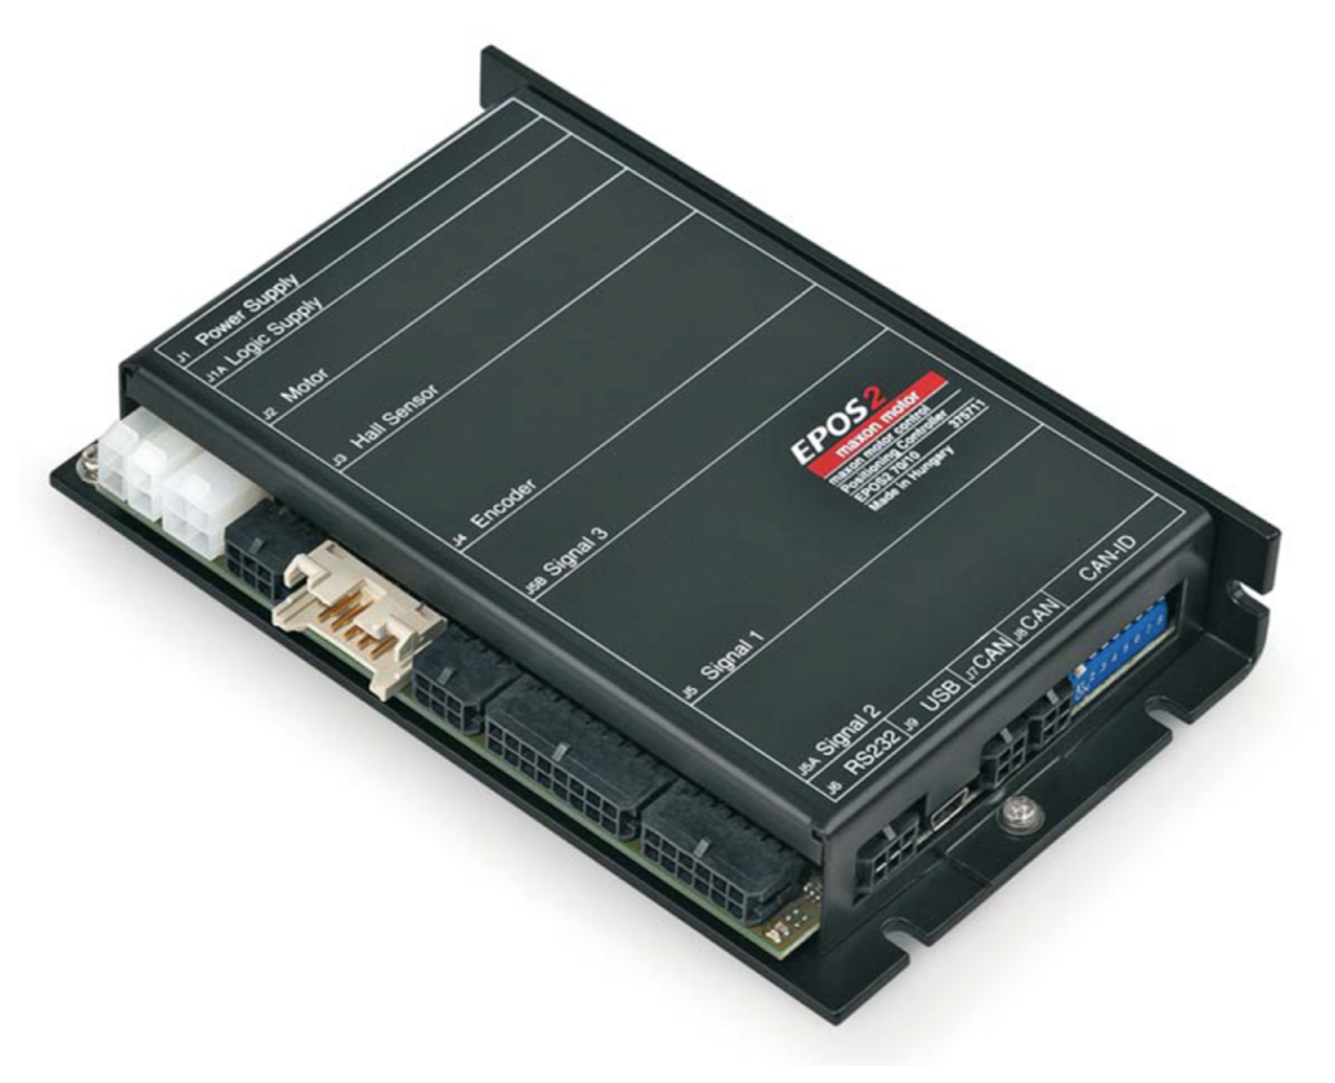
\includegraphics[height=40mm]{figure/epos.eps}
      \vspace*{3mm}
      \caption{EPOS2 70/10(375711)}
    \label{fig:epos}
    \end{center}
  \end{minipage}
  \begin{minipage}{0.6\textwidth}
      \begin{center}
	\makeatletter
	\def\@captype{table}   
	\makeatother
	\caption{Specification of EPOS2 70/10(375711)}
	\label{tab:epos}
	\begin{tabular}{cc}\hline
	  power suppy voltage [VDC] & 11-70\\
	  Max output current [A] & 25\\
	  Max continuous current [A] & 10\\
	  Hall sensor & H1, H2, H3 \\
	  Encoder & A, A$\setminus$, B, B$\setminus$, I, I$\setminus$(max. 5MHz)\\
	  Analog Input & 2(differential, 12-bit, 0...+5 V)\\
	  RS232 & RxD; TxD(max. 115200 bit/2) \\\hline 
	  \end{tabular}  
	\end{center}
  \end{minipage}
\end{figure}

\vspace*{10mm}
\begin{figure}[htp]
  \begin{center}
    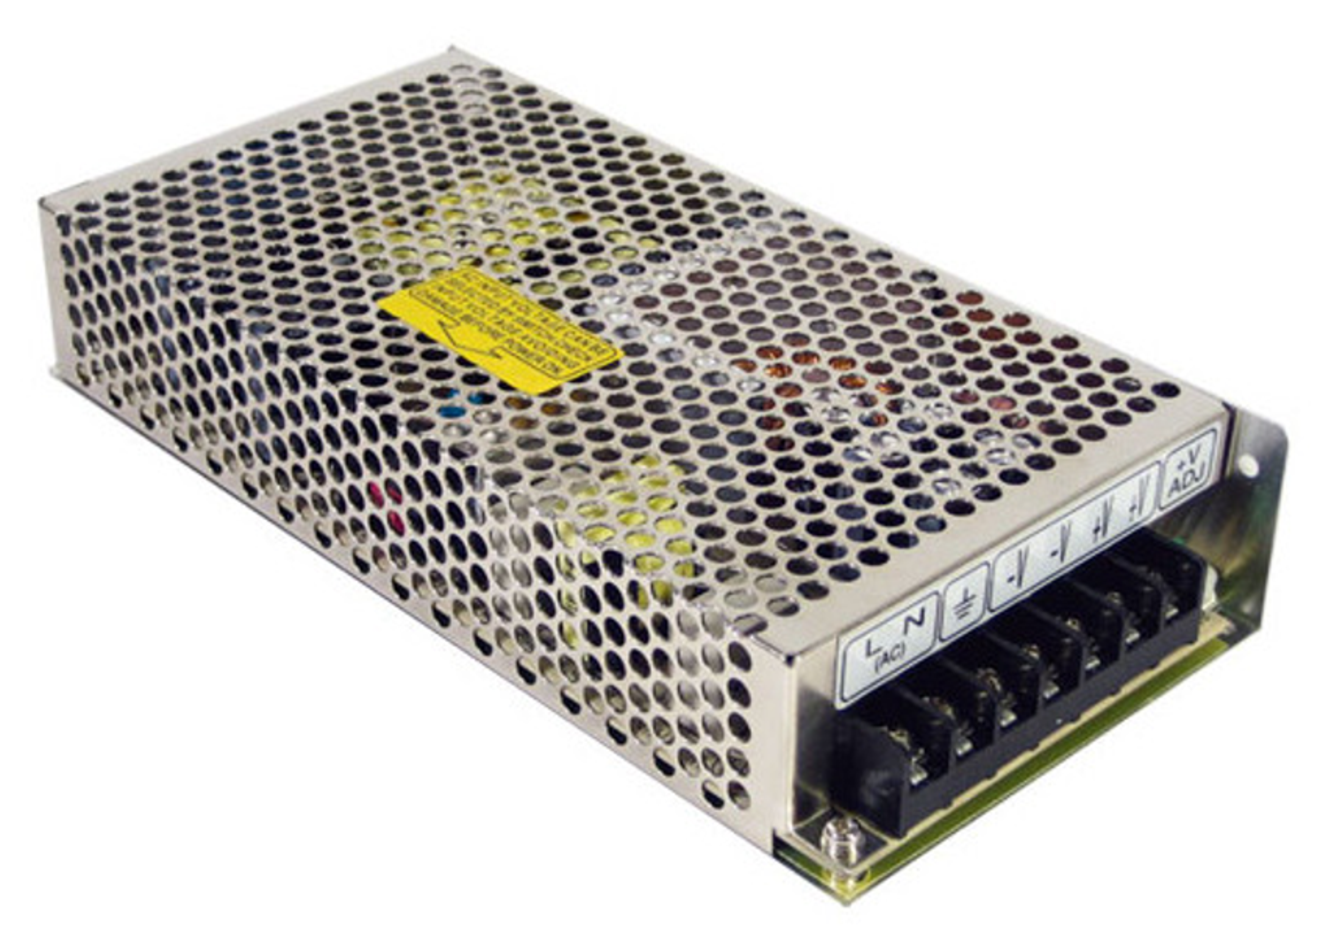
\includegraphics[height=40mm]{figure/rs_150_24.eps}
    \vspace*{3mm}
    \caption{Swiching Power Supply(RS-150-24)}
    \label{fig:rs_150_24}
  \end{center}
\end{figure}

\newpage
本研究では、シリアル通信を用いて位置制御を行った。それにあたり、RS232ケーブルを用いてPC-PC間でシリアル通信を用いて値を送り、モータドライバの使用方法を確認した。送信に使用したSimulinkを図~\ref{fig:serial_send}~、受信に使用したSimulinkを図~\ref{fig:serial_recieve}~に示す。通信周期は2msで行った。シリアル通信を行う際、表~\ref{tab:serial}~に示すような設定が必要であり、Simulinkの「Serial Configration」ブロックを用いて設定した。図~\ref{fig:serial_send}~にある「MATLAB Function」ブロックは付録に示す。これは、ETH Zurich(スイス連邦工科大学チューリッヒ校)のAutonomous Systems Laboratoryが公開しているGitHub(ethz-asl/matlab-epos-librery)を参考にした。\cite{99}

\vspace*{10mm}
\begin{figure}[htp]
  \begin{center}
    \includegraphics[height=40mm]{figure/serial_send.eps}
    \vspace*{3mm}
    \caption{Serial Send}
    \label{fig:serial_send}
  \end{center}
\end{figure}

\vspace*{10mm}
\begin{figure}[htp]
  \begin{center}
    \includegraphics[height=60mm]{figure/serial_recieve.eps}
      \vspace*{3mm}
      \caption{Serial Recieve}
      \label{fig:serial_recieve}
  \end{center}
\end{figure}

\newpage
\begin{table}[htp]
  \begin{center}
    \makeatletter
    \def\@captype{table}   
    \makeatother
    \caption{Specification of Serial Communication(RS232)}
      \label{tab:serial}
	\begin{tabular}{cc}\hline
	  Parameter & Value\\\hline
	  Baud Rate & 115200 [bps]\\ 
	  Start Bits & 1\\
	  Data Bits & 8\\
	  Parity & none\\ 
	  Stop Bits & 1\\
	  Byte Order & Little Endian\\
	  Terminator & $\backslash$n\\\hline
      \end{tabular}  
    \end{center}
\end{table}

\vspace*{10mm}
このモータドライバと路面部モータであるECブラシレスモータ「EC22 386658」を用いて位置制御の確認を行った。モータドライバ「EPOS2 70/10 375711」はmaxon motor社製のグラフィカル・ユーザ・インターフェース「EPOS Studio」を用いて、モータやエンコーダなどにモータドライバが適合するようにシステム設定を行うことができる。\cite{22}また、制御ゲインのオート・チューニング機能を用いて、電流、速度、位置の制御ゲインを自動的に調整している。図~\ref{fig:serial_send}~の送信先をモーダドライバに設定した。オシロスコープを使って通信が正常に行われていることと、モータが動作することを確認した。なお、オシロスコープでは通信周期の2msごとに0Vと1Vに切り替わる矩形波を見ることができる。図~\ref{fig:epos_studio}~に「EPOS Studio」の画面を示す。

\vspace*{10mm}
\begin{figure}[htp]
  \begin{center}
    \includegraphics[height=80mm]{figure/epos_studio.eps}
    \vspace*{3mm}
    \caption{EPOS Studio}
    \label{fig:epos_studio}
  \end{center}
\end{figure}

% **************************************************
\newpage
\subsection{計測機器}
\subsubsection{1軸ロードセル}
ダンパが発生する力の計測には図~\ref{fig:tclz}~に示す東京測器研究所の引張・圧縮型高精度荷重計「TCLS-20NA」を用いた.仕様を表~\ref{tab:tclz}~に示す.このロードセルをダンパとばね上の間に取り付けることでダンパ力を計測する.ロードセルから出力された電圧値は,東京測器研究所のデジタル指示計「TD-96A」を用いて換算する.このデジタル指示計は,ひずみゲージ式変換器を用いて荷重,変位,圧力などを測定できる.外観を図~\ref{fig:td_96a}~に,仕様を表~\ref{tab:td_96a}~に示す.

\vspace*{10mm}
\begin{figure}[h!]
  \begin{tabular}{cc}
  \begin{minipage}{0.5\hsize}
  \begin{center} 
    \includegraphics[height=40mm]{figure/tclz.eps}
      \vspace*{3mm}
      \caption{Loadcell(TCLZ-20NA)}
      \label{fig:tclz}
    \end{center}
  \end{minipage}
  \begin{minipage}{0.5\hsize}
     \begin{center}
      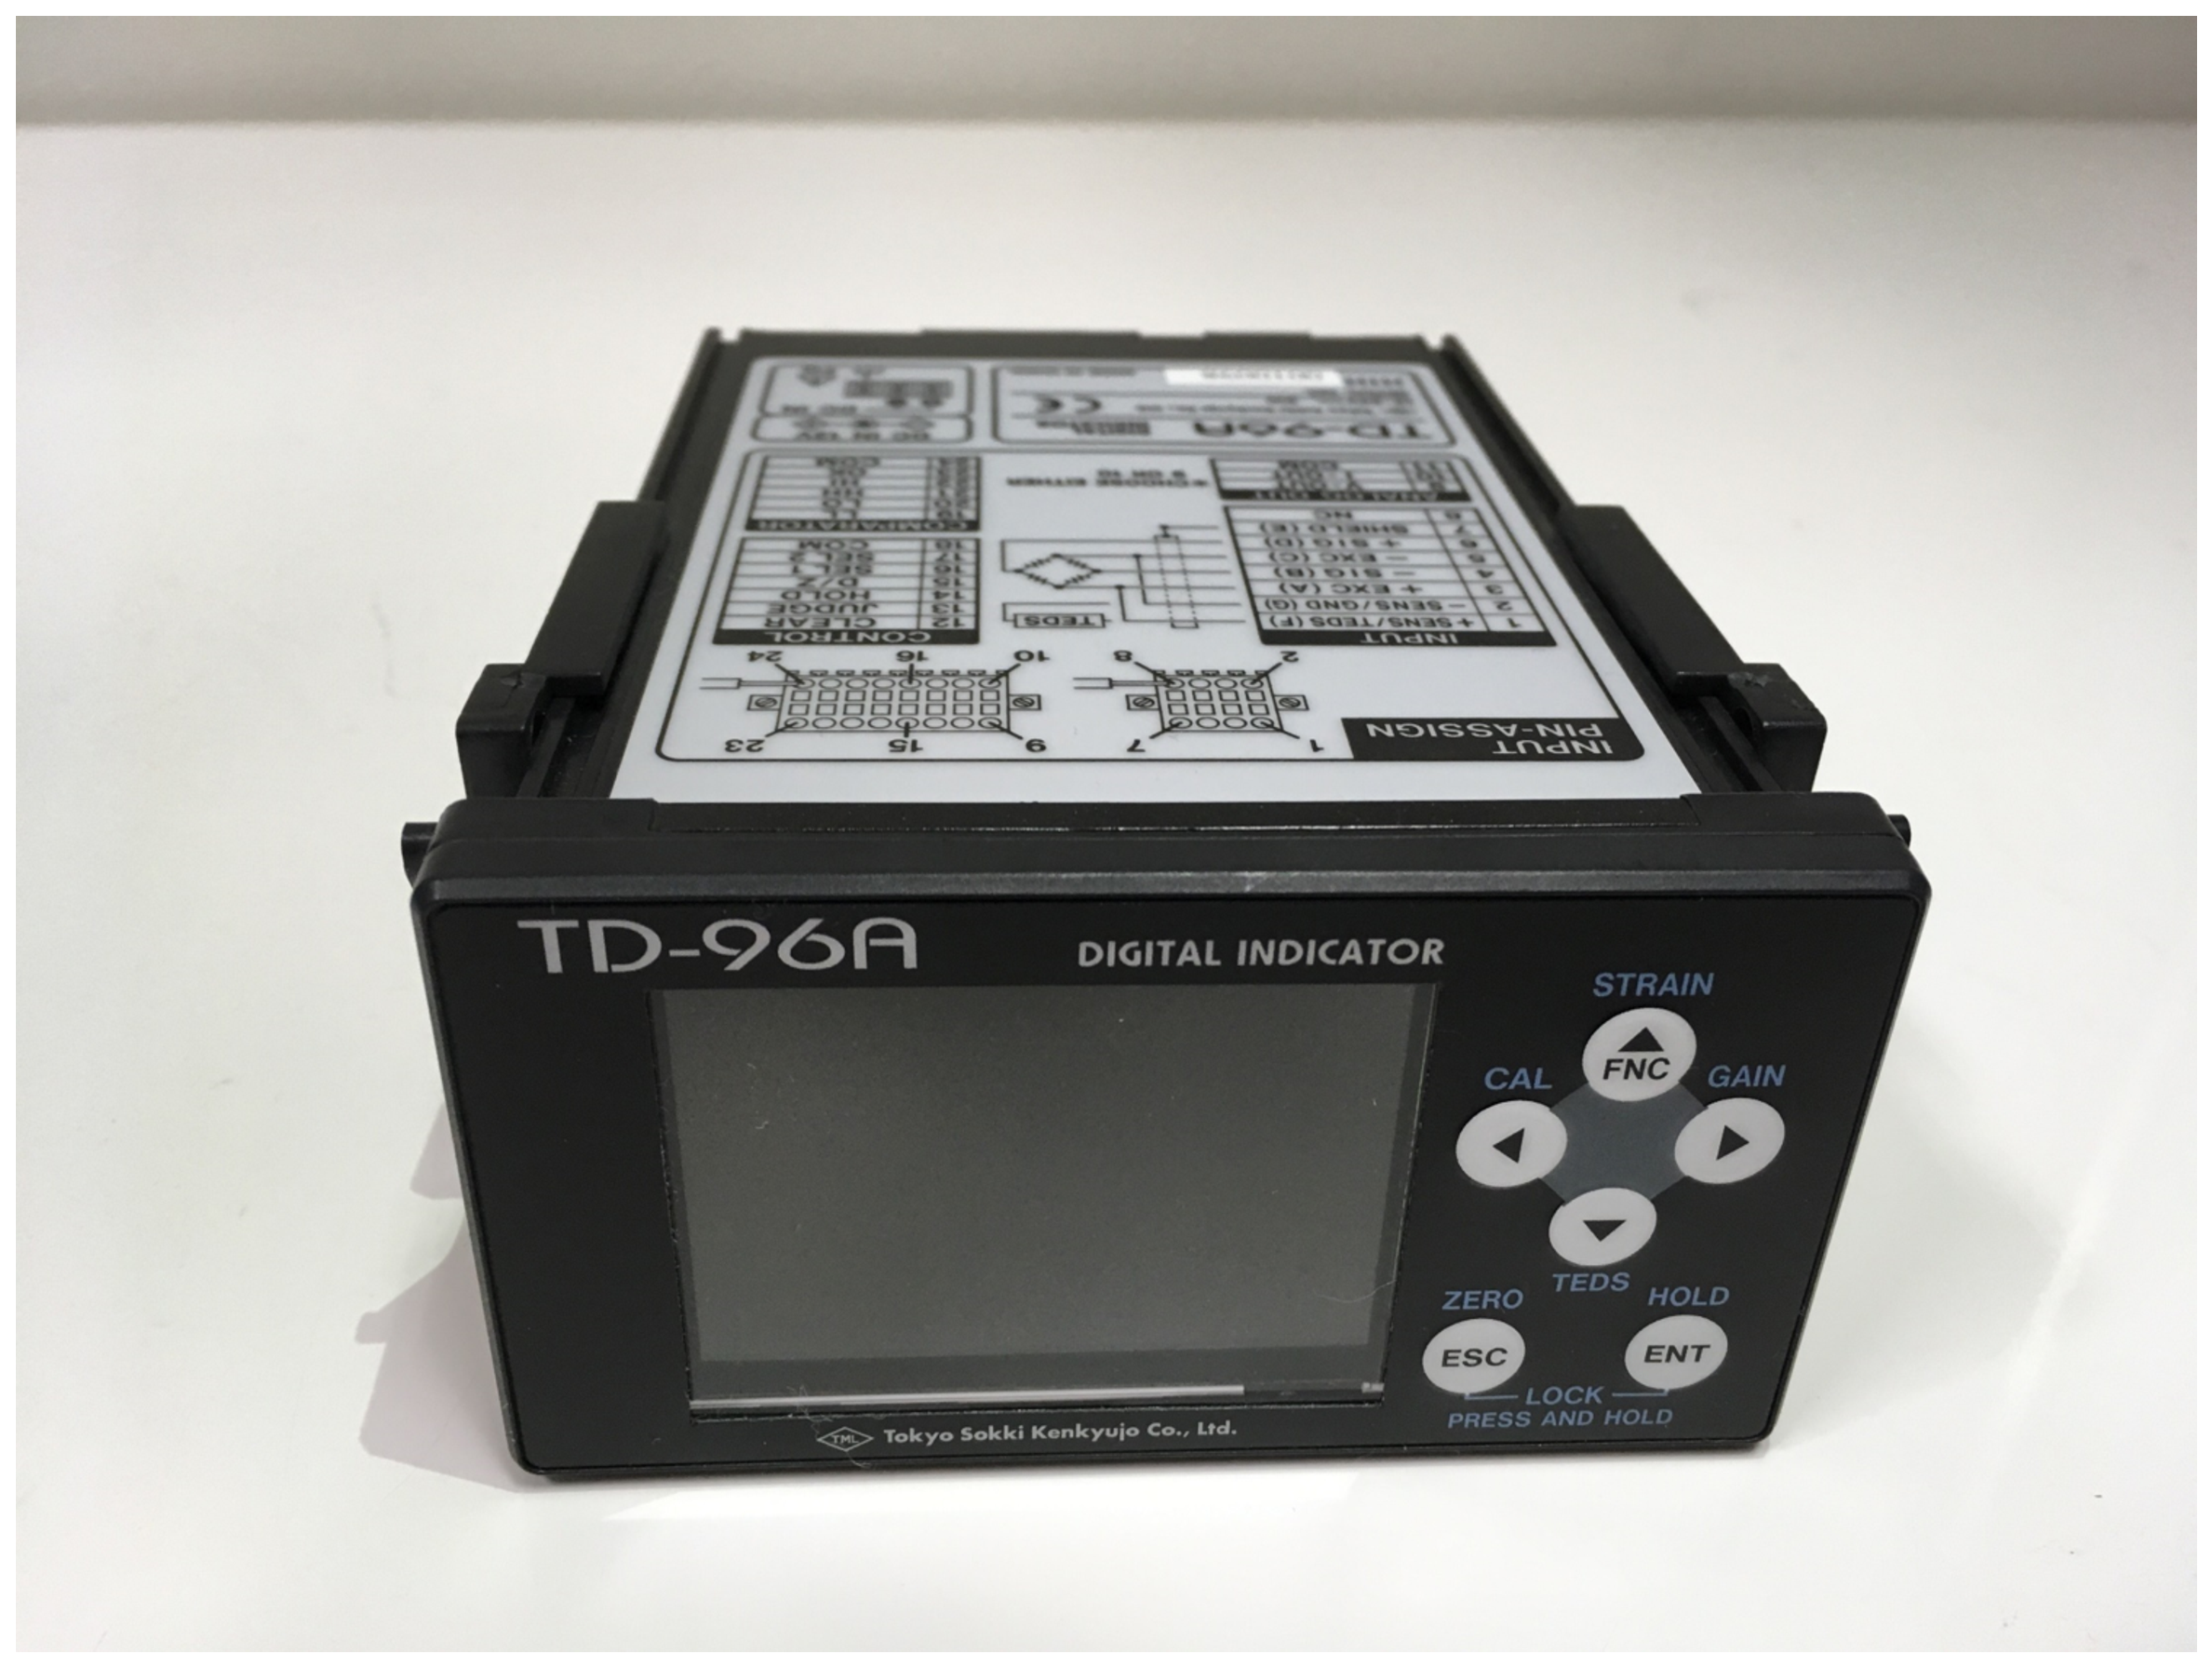
\includegraphics[height=40mm]{figure/td_96a.eps}
      \vspace*{3mm}
      \caption{Digital Indictor(TD-96A)}
      \label{fig:td_96a}
    \end{center}
  \end{minipage}
  \end{tabular}
 \end{figure}

\vspace*{10mm}
\begin{table}[h]
  \begin{center}
    \caption{Specification of Loadcell}
	\label{tab:tclz}
	\begin{tabular}{crrc}\hline
	  Parameter & \multicolumn{2}{c}{Value}&\\\hline
	  Capacity & \multicolumn{2}{c}{20 N}&\\
	  Overload Capacity & \multicolumn{2}{c}{30N}&\\
	    & Ten.&Comp.\\
	  Rated Output & +1248.7 & -1248.4 & $\mu$V/V \\ 
	  Strain & +2497.3 & -2496.8 & $\times$ 10$^-6$ $\epsilon$ \\
	  Calibration Coefficient & 0.008009 & 0.008010 & N/1$\times$ 10$^-6$ \\\hline
	\end{tabular}
  \end{center}
\end{table}

\vspace*{10mm}
\begin{table}[h]
  \begin{center}
    \caption{Specification of TD-96A}
    \label{tab:td_96a}
    \begin{tabular}{cc}\hline
      Measurement Point & 1 \\
      Measurement Range [mV/V]& $\pm$3\\
      A/D Conversion Speed [Hz]& 4000\\
      D/A Output [mA]& 0$\pm$1$\sim\pm$10 V, 4$\sim$20\\
      Power supply & AC100 V 12 W, DC12$\sim$24 V 9 W \\\hline 
    \end{tabular}
  \end{center}
\end{table}

% --------------------------------------------------
\newpage
\subsubsection{レーザ変位計}
ばね下変位の計測には図~\ref{fig:il_300}~に示す株式会社KEYENCEのセンサヘッド「IL-300」を用いた.仕様を表~\ref{tab:il_300}~に示す.出力電圧は±5V,1-5V,0-5Vから選択できる.計測距離をL[mm],アナログ出力電圧をV[V]とした時,換算式はそれぞれ以下のようになる.本研究では,出力電圧±5Vの式~\ref{eq:v5}~を用いた.また,アンプとして,図~\ref{fig:il_1500}~に示す株式会社KEYENCEのアンプユニット「IL-1500」を用いた.アンプユニットには,図~\ref{fig:kz_u3}~に示す株式会社KEYENCEのAC電源ユニット「KZ-U3」を用いて24Vの直流電圧を供給している.

\begin{eqnarray}
 \label{eq:v5} L &=& V_{\pm5V} \times 28\\
 \label{eq:v15} L &=& V_{1-5V} \times 70\\
 \label{eq:v05} L &=& V_{0-5V} \times 56
\end{eqnarray}

\vspace*{10mm}
\begin{figure}[htp]
  \begin{minipage}{0.3\textwidth}
    \begin{center}
      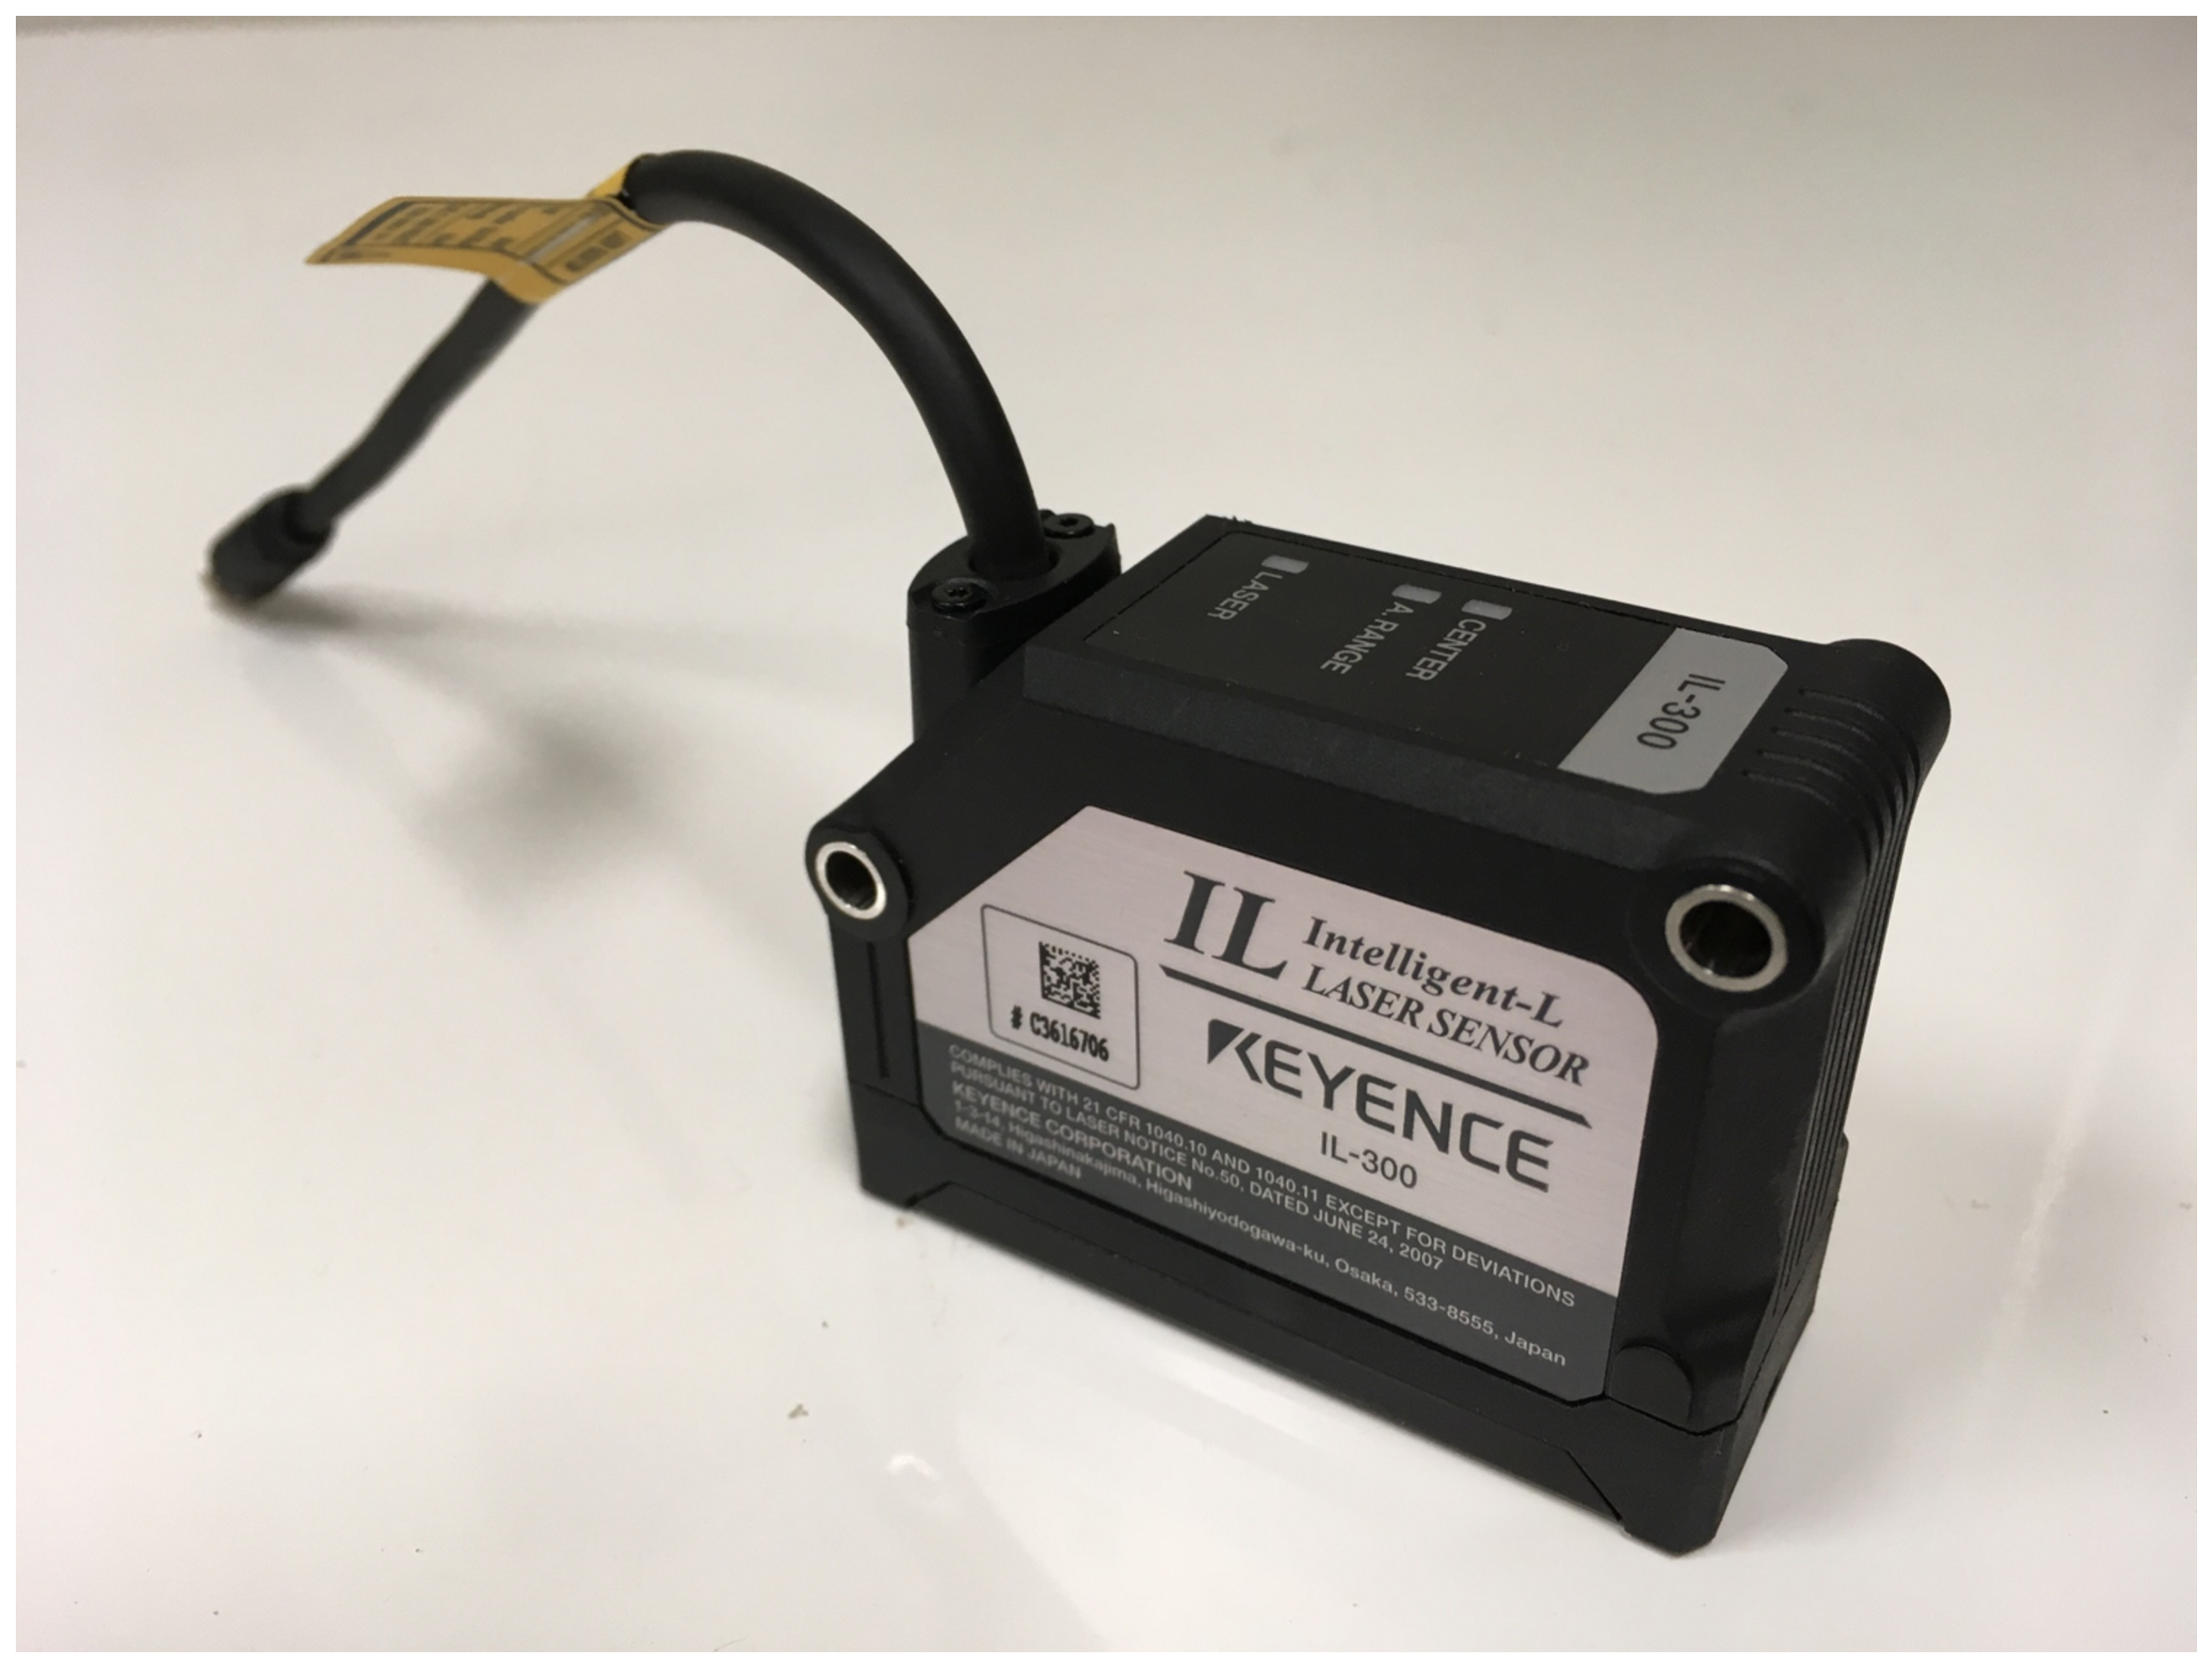
\includegraphics[height=40mm]{figure/il_300.eps}
      \vspace*{3mm}
      \caption{Laser Displacement Sensor(IL-300)}
      \label{fig:il_300}
    \end{center}
  \end{minipage}
  \begin{minipage}{0.7\textwidth}
      \begin{center}
	\makeatletter
	\def\@captype{table}   
	\makeatother
	\caption{Specification of Laser Displacement Sensor}
	\label{tab:il_300}
	\begin{tabular}{ccc}\hline
	  Measurement Center Distance [mm] & 300\\
	  Measuring Range & 160-450 mm\\
	  Sampling Period [$\mu$s]& 0.33 / 1 / 2 / 5\\
	  Resolition [$\mu$m] & 10\\
	  Linearity [\%F.S.] & $\pm$0.25\\
	  Receiving Element & Liner Image Sensor\\
	  Resistance to Vibration [Hz] & 10-55\\
	  Laser Class & 2\\
	  Power Supply & DC10-30 V\\\hline 
	  \end{tabular}  
	\end{center}
  \end{minipage}
\end{figure}

\vspace*{10mm}
\begin{figure}[htp]
  \begin{minipage}{0.5\textwidth}
    \begin{center}
      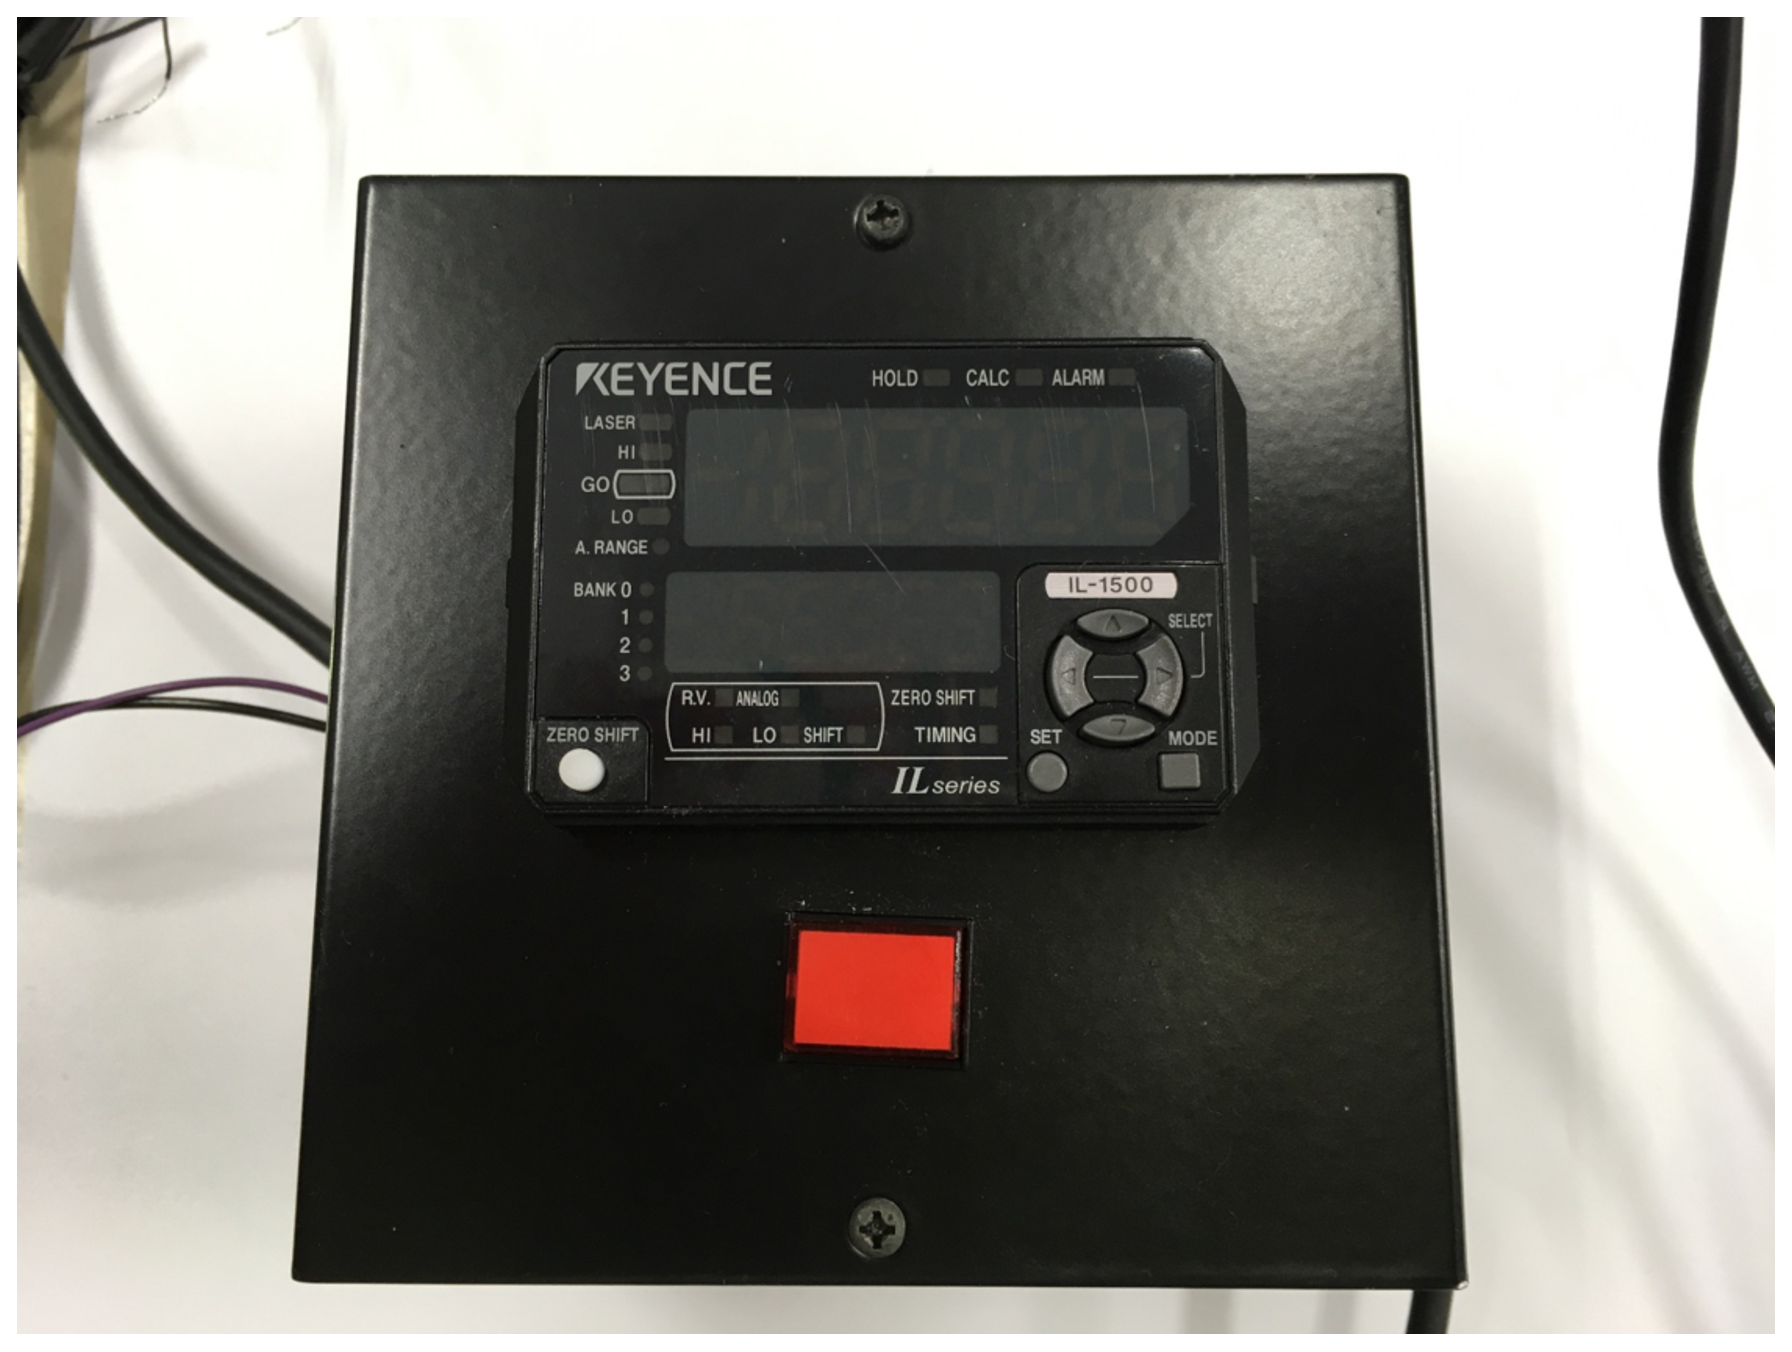
\includegraphics[height=40mm]{figure/il_1500.eps}
      \vspace*{3mm}
      \caption{Amplifier Unit(IL-1500)}
      \label{fig:il_1500} 
    \end{center}
  \end{minipage}
  \begin{minipage}{0.5\textwidth}
    \begin{center}
      \includegraphics[height=40mm]{figure/kz_u3.eps}
      \vspace*{3mm}
      \caption{Power Supply Unit(KZ-U3)}
      \label{fig:kz_u3}  
    \end{center}
  \end{minipage}
\end{figure}

% **************************************************
\newpage
\subsection{ソフトウェア部}
\subsubsection{dSPACEシステム}
本システムでは,dSPACE社製の開発環境であるdSPACEシステムを利用している.上下変位計算とハードウェア制御にはdSPACE社製のController Board「DS1104 Controller Board」を使用している.Controller Boardを図~\ref{fig:ds1104}~に,Connector Panelを図~\ref{fig:conpane}~に示す.Controller Boardは,デジタル入出力用チャンネル,A/Dコンバータ用チャンネル,D/Aコンバータ用チャンネルを備えており,多くの用途に対応できる.また,Digital Incremental Encorder Interface用チャンネルによるエンコーダの計測や,Serial Interfaceに対応しておりボーレート最大115200bpsのRS232通信が可能である.

\vspace{10mm}
\begin{figure}[h]
    \begin{tabular}{c}
      \begin{minipage}{0.5\hsize}
	\begin{center}
	  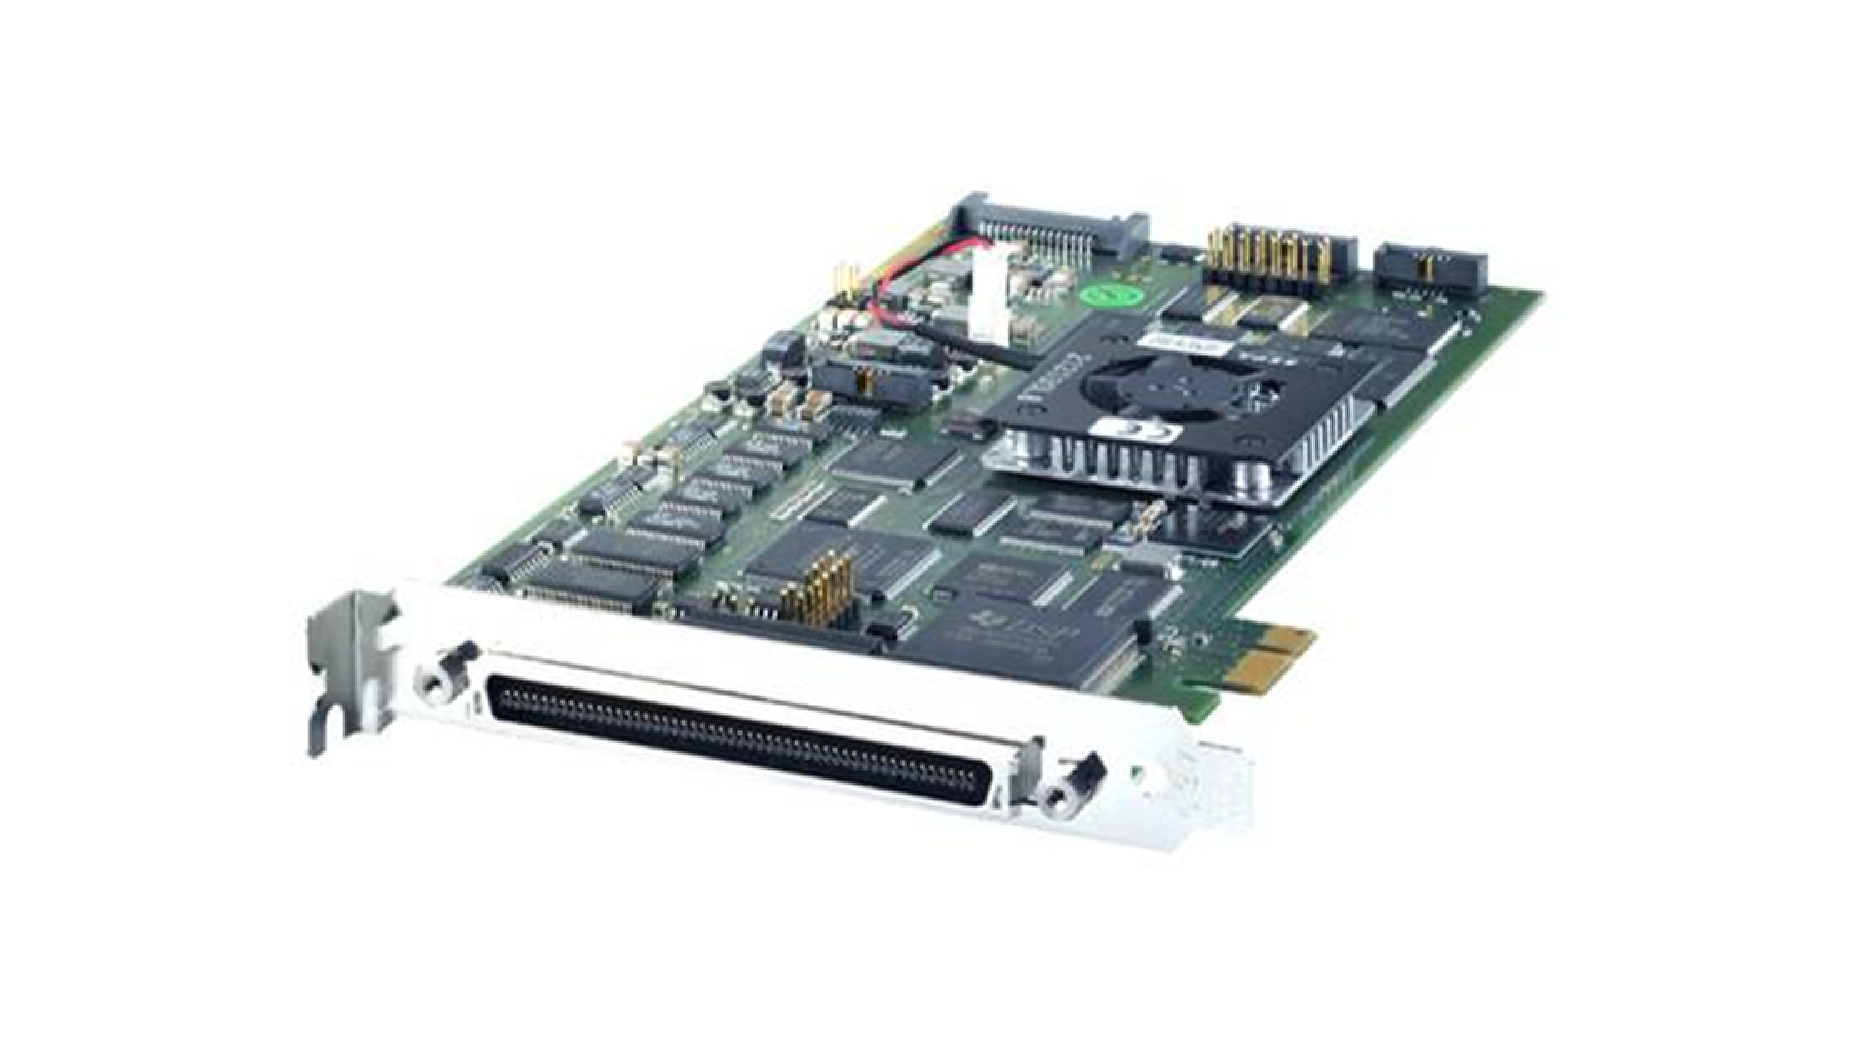
\includegraphics[height=25mm]{figure/ds1104.eps}
	  \caption{Controller Borad\cite{6}}
	  \label{fig:ds1104}
	\end{center}
      \end{minipage}
      \begin{minipage}{0.5\hsize}
	\begin{center}
	  \includegraphics[height=25mm]{figure/conpane.eps}
	  \caption{Connector Panel\cite{6}}
	  \label{fig:conpane}
	\end{center}
      \end{minipage}
    \end{tabular}
\end{figure}

\vspace{10mm}
Real-Time Interfaceは,dSPACE社製のハードウェアとMathWorks社製のソフトウェア「MATLAB /Simulink」の間のリンクとなるものである.これにより,Simulinkモデルを用いてdSPACEシステムの入出力機器と信号処理を行うことができる.また,MATLAB/Simulinkで作成されたモデルは,Simulink Corderにより,実時間で実行可能なCコードに変換され,Controller Board上で実行される.このような開発環境を構築することで,実時間シミュレーションを行うHILSシステムを実現している.制御インターフェースとしては,dSPACE社製のControl Deskを用いている.「MATLAB/Simulink」と関連付けることで,試験条件の設定やハードウェアへの指令値,計測値,車両運動解析の結果をモニタリングできる.また,リアルタイムで計測値や解析結果をグラフとして描画できる.図~\ref{fig:control_desk}~では指令値や計測値,上下変位計算の結果を表示したControl Deskの画面である.

 \vspace{10mm}
\begin{figure}[h]
  \centering
  \includegraphics[height=30mm]{figure/control_desk.eps}
  \vspace{2mm}
   \caption{Control Desk}
  \label{fig:control_desk}
\end{figure}

% **************************************************
\newpage
\subsection{解析モデル}
本システムにおいて解析モデルは上下2自由度モデルを用いた.上下2自由度モデルは車両の上下動を表すことのできるモデルのひとつである\cite{7}.モデル図を図~\ref{fig:analysis_model}~に,諸元を表~\ref{tab:parameter}~に示す.また,このモデルの運動方程式は以下である.

\begin{eqnarray}
 \label{eq:2dof_m1} &&m_1\ddot x_1 + c_2(\dot x_1-\dot x_2) + k_1(x_1-x_0) + k_2(x_1-x_2) = 0\\
 \label{eq:2dof_m2} &&m_2\ddot x_2 + c_2(\dot x_2-\dot x_1) + k_2(x_2-x_1) = 0
\end{eqnarray}

\vspace{10mm}
ここで,$m_1$はばね下質量 ,$m_2$はばね上質量,$k_1$,$k_2$はばね定数,$c_2$は減衰係数,$x_0$は路面変位,$x_1$はばね下変位,$x_2$はばね上変位である.減衰比$\zeta$と減衰係数$c_2$の関係は式~\ref{eq:zeta}~で表される.

\vspace{10mm}
\begin{eqnarray}
 \label{eq:zeta} \zeta = \frac{c}{2\sqrt{mk}}
\end{eqnarray}

\vspace*{10mm}
\begin{figure}[htp]
  \begin{minipage}{0.5\textwidth}
    \begin{center}
      \includegraphics[height=40mm]{figure/analysis_model.eps}
      \vspace*{3mm}
      \caption{Analysis Model}
      \label{fig:analysis_model}
    \end{center}
  \end{minipage}
  \begin{minipage}{0.5\textwidth}
      \begin{center}
	\makeatletter
	\def\@captype{table}   
	\makeatother
	\caption{Parameter of Analysis Model}
	\label{tab:parameter}
	  \begin{tabular}{cc}\hline
	    Unsprung Mass $m_1$ [kg] & 1.2\\
	    Sprung Mass $m_2$ [kg] & 6.4\\
	    Spring constant $k_1$ [N/m] & 2200\\
	    Spring constant $k_2$ [N/m] & 405\\
	    Damping coefficient $c_2$ [N/m] & 30\\\hline 
	  \end{tabular}  
	\end{center}
  \end{minipage}
\end{figure}

% #################################################
\newpage
\section{上下動再現手法の検討}
\subsection{1自由度系HILSシステム}
1自由度系HILSシステムのブロック線図を図~\ref{fig:1dof_block}~に,ハードウェアのモデルを図~\ref{fig:1dof_hardware}~に示す.1自由度系のハードウェア部は,試験装置のばね上を固定することで再現する.ハードウェアから計測されたダンパ力を用いてリアルタイムに車両運動解析を実行し,ばね上-ばね下間相対変位$x_2-x_1$を算出する.モータへの入力$\bar x_0$は,解析モデルを用いて計算したばね上-路面間相対変位$x_2-x_0$に基づき決定する.解析モデルのばね上-ばね下間相対変位$x_2-x_1$は試験装置の$-\bar x_1$に相当する.そこで,試験装置を図~\ref{fig:1dof_hardware}~に示すような1自由度振動系してモデル化し,入力$\bar x_0$に対するばね上-ばね下間相対変位$-\bar x_1$の伝達関数を求め,その逆伝達関数を用いることでモータへの入力を決定する.1自由度振動系の運動方程式は以下である.

\vspace{-5mm}
\begin{eqnarray}
 \label{eq:1dof_m1} m_1\ddot{\bar x}_1 + c_2\dot{\bar x}_1 + k_1(\bar x_1-\bar x_0) + k_2\bar x_1 = 0
\end{eqnarray}

ここで,$m_1$はばね下質量 ,$k_1$,$k_2$はばね定数,$c_2$は減衰係数,$\bar x_0$は路面変位,$\bar x_1$はばね下変位である.この1自由度系HILSシステムの場合,ハードウェアへの入力が1つであるため,装置としては扱いやすくなる.しかし,モータは装置の荷重を支えつつ高い応答性を要求される.

\vspace*{10mm}
\begin{figure}[htp]
  \begin{center}
    \includegraphics[height=20mm]{figure/1dof_block.eps}
    \vspace*{3mm}
    \caption{Block Diagram(1DOF)}
    \label{fig:1dof_block}
  \end{center}
\end{figure}

\vspace*{10mm}
\begin{figure}[htp]
  \begin{center}
    \includegraphics[height=40mm]{figure/1dof_hardware.eps}
    \vspace*{3mm}
    \caption{Hardware Model(1DOF)}
    \label{fig:1dof_hardware}
  \end{center}
\end{figure}

% **************************************************
\newpage
\subsection{2自由度系HILSシステム}
2自由度系HILSシステムのブロック線図を図~\ref{fig:2dof_block}~に,ハードウェアのモデルを図~\ref{fig:2dof_hardware}~に示す.ハードウェアには2つのモータを用いて,ばね上変位$x_2$と路面変位$x_0$をそれぞれ入力する.ハードウェアから計測されたダンパ力を用いてリアルタイムに車両運動解析を実行し,その結果に基づきばね上変位$x_2$を制御する.この2自由度HILSシステムの場合,荷重を支える路面部のモータと,リアルタイム解析の結果に基づいた制御を行うばね上のモータに役割を分けることができる.しかし,モータが2つであるため,試験装置の取り扱いが複雑になる.

\vspace*{10mm}
\begin{figure}[htp]
  \begin{center}
    \includegraphics[height=30mm]{figure/2dof_block.eps}
    \vspace*{3mm}
    \caption{Block Diagram(2DOF)}
    \label{fig:2dof_block}
  \end{center}
\end{figure}

\vspace*{10mm}
\begin{figure}[htp]
  \begin{center}
    \includegraphics[height=50mm]{figure/2dof_hardware.eps}
    \vspace*{3mm}
    \caption{Hardware Model(2DOF)}
    \label{fig:2dof_hardware}
  \end{center}
\end{figure}

% **************************************************
\newpage
\subsection{構築したHILSシステムの有用性の確認}
構築した2種類のHILSシステムに対して,図~\ref{fig:step_6_input}~に示すステップ入力を与え,HILSシステムの有用性を確認した.図~\ref{fig:1_wo_feedback}~から図~\ref{fig:2_with_feedback}~は,1自由度系と2自由度系それぞれについて,ダンパ力をフィードバックせずにモータを制御した際のばね上-ばね下間相対変位と,ダンパ力の計測結果に基づき車両運動解析を実行し,モータを制御した際のばね上-ばね下間相対変位を比較したグラフである.ダンパ力の計測結果には50Hz、ばね上-ばね下間相対変位の計測結果には100Hzのローパスフィルタをかけてある。(a)と(b)を比較すると,ダンパ力をフィードバックすることによって解析結果が変化することが確認できる.このことから,ダンパ力をフィードバックすることによって,ダンパの非線形性を考慮でき,ばね上-ばね下間相対変位の再現性が向上したといえる.\par
図~\ref{fig:1_with_feedback}~をみると,ステップ入力が入った直後に高周波な振動が現れていることがわかる.これは図~\ref{fig:iida}~に示した車体部のばねの固有振動数が現れていると考えられる.ばねの質量は付録の要目表から0.991kgであり,試験装置に対して無視できない大きさである.なお,この現象は目視で確認できる程度のものであり,2自由度系HILSシステムでも同様の現象がみられた.

\vspace*{10mm}
\begin{figure}[htp]
  \begin{center}
    \includegraphics[scale=1]{figure/step_6_input.eps}
    \vspace*{3mm}
    \caption{Road Input}
    \label{fig:step_6_input}
  \end{center}
\end{figure}

\newpage
\begin{figure}[htp]
  \begin{tabular}{cc}
  \begin{minipage}{0.5\hsize}
  \begin{center} 
    \includegraphics[scale=1]{figure/1_open_step_6.eps}
    \end{center}
    \begin{center}
    \vspace*{3mm}
    \ (a)Suspension Stroke\
%     \label{fig:1_open_step_6} 
    \end{center}
  \end{minipage}
  \begin{minipage}{0.5\hsize}
     \begin{center}
      \includegraphics[scale=1]{figure/1_open_step_6_damp.eps}
      \end{center}
      \begin{center}
      \vspace*{3mm}
      \ (b)Damper Force to use for Analysis\
%       \label{fig:1_open_step_6_damp}
    \end{center}
  \end{minipage}
  \end{tabular}
  \vspace*{3mm}
  \caption{w/o Feedback(1DOF)}
    \label{fig:1_wo_feedback}
\end{figure}

\vspace*{10mm}
\begin{figure}[htp]
  \begin{tabular}{cc}
  \begin{minipage}{0.5\hsize}
  \begin{center} 
    \includegraphics[scale=1]{figure/1_close_step_6.eps}
    \end{center}
    \begin{center}
    \vspace*{3mm}
    \ (a)Suspension Stroke\
%     \label{fig:1_close_step_6} 
    \end{center}
  \end{minipage}
  \begin{minipage}{0.5\hsize}
     \begin{center}
      \includegraphics[scale=1]{figure/1_close_step_6_damp.eps}
      \end{center}
      \begin{center}
      \vspace*{3mm}
      \ (b)Damper Force to use for Analysis\
%       \label{fig:1_close_step_6_damp}
    \end{center}
  \end{minipage}
  \end{tabular}
  \vspace*{3mm}
  \caption{with Feedback(1DOF)}
    \label{fig:1_with_feedback}
\end{figure}

\newpage
\begin{figure}[htp]
  \begin{tabular}{cc}
  \begin{minipage}{0.5\hsize}
  \begin{center} 
    \includegraphics[scale=1]{figure/2_open_step_6.eps}
    \end{center}
    \begin{center}
    \vspace*{3mm}
    \ (a)Suspension Stroke\
%     \label{fig:2_open_step_6} 
    \end{center}
  \end{minipage}
  \begin{minipage}{0.5\hsize}
     \begin{center}
      \includegraphics[scale=1]{figure/2_open_step_6_damp.eps}
      \end{center}
      \begin{center}
      \vspace*{3mm}
      \ (b)Damper Force to use for Analysis\
%       \label{fig:2_open_step_6_damp}
    \end{center}
  \end{minipage}
  \end{tabular}
  \vspace*{3mm}
  \caption{w/o Feedback(2DOF)}
    \label{fig:2_wo_feedback}
\end{figure}

\vspace*{10mm}
\begin{figure}[htp]
  \begin{tabular}{cc}
  \begin{minipage}{0.5\hsize}
  \begin{center} 
    \includegraphics[scale=1]{figure/2_close_step_6.eps}
    \end{center}
    \begin{center}
    \vspace*{3mm}
    \ (a)Suspension Stroke\
%     \label{fig:2_close_step_6} 
    \end{center}
  \end{minipage}
  \begin{minipage}{0.5\hsize}
     \begin{center}
      \includegraphics[scale=1]{figure/2_close_step_6_damp.eps}
      \end{center}
      \begin{center}
      \vspace*{3mm}
      \ (b)Damper Force to use for Analysis\
%       \label{fig:2_close_step_6_damp}
    \end{center}
  \end{minipage}
  \end{tabular}
  \vspace*{3mm}
  \caption{with Feedback(2DOF)}
    \label{fig:2_with_feedback}
\end{figure}

% **************************************************
\newpage
\subsection{HILSシステムにおける上下動再現手法の検討}
1自由度系HILSシステムと2自由度系HILSシステムにおける上下動の再現性を評価するために,路面入力試験を行った.図~\ref{fig:compare_2_7}~に周波数2.0Hz,振幅7mmの正弦波を路面に入力した際の,サスペンションストロークを比較したグラフを示す.入力周波数が低い場合は,解析結果とハードウェアの計測値が同じ挙動を示したため,上下動の再現性は高いと言える.しかし,図~\ref{fig:compare_2_7}~(a) の1自由度系HILSシステムでは,解析結果に対して計測値が僅かに遅れていることがわかる.1自由度系HILSシステムでは4.1節で述べたように,ハードウェアの逆伝達関数を用いてアクチュエータの入力を決定している.ハードウェアの逆伝達関数には微分の項が含まれる.微分をすると系が不安定になるため,3次のローパスフィルタをかけてある.カットオフ周波数は50Hzである.図~\ref{fig:compare_2_7}~(a)からわかる遅れは,このローパスフィルタによるものであると考えられる.\par

\vspace*{10mm}
\begin{figure}[h]
  \begin{tabular}{cc}
  \begin{minipage}{0.5\hsize}
  \begin{center} 
    \includegraphics[scale=1]{figure/1_close_sine_2_7.eps}
    \end{center}
    \begin{center}
    \vspace*{3mm}
    \ (a)1DOF HILS\
%     \label{fig:1_close_sine_2_7} 
    \end{center}
  \end{minipage}
  \begin{minipage}{0.5\hsize}
     \begin{center}
      \includegraphics[scale=1]{figure/2_close_sine_2_7.eps}
      \end{center}
      \begin{center}
      \vspace*{3mm}
      \ (b)2DOF HILS\
%       \label{fig:2_close_sine_2_7}
    \end{center}
  \end{minipage}
  \end{tabular}
  \vspace*{3mm}
  \caption{Comparison of Suspension Stroke(Input:2Hz 7mm)}
    \label{fig:compare_2_7}
\end{figure}

\newpage
図~\ref{fig:compare_5_2}~に周波数5Hz,振幅2mmの正弦波を路面に入力した際の,サスペンションストロークを比較したグラフを示す.入力周波数が高くなると,特に1自由度系HILSシステムで解析結果と計測値の振幅が離れた.これは図~\ref{fig:compare_2_7}~の場合と同様に,解析モデルとハードウェアの動特性が異なるためであると考えられる.また,アクチュエータの応答性が影響したことも考えられる.モータ単体の周波数応答は確認したが,装置を組み立てて,モータに負荷がかかった際に周波数応答特性が変化した可能性が挙げられる.

\vspace*{10mm}
\begin{figure}[h]
  \begin{tabular}{cc}
  \begin{minipage}{0.5\hsize}
  \begin{center} 
    \includegraphics[scale=1]{figure/1_close_sine_5_2.eps}
    \end{center}
    \begin{center}
    \vspace*{3mm}
    \ (a)1DOF HILS\
%     \label{fig:1_close_sine_5_2} 
    \end{center}
  \end{minipage}
  \begin{minipage}{0.5\hsize}
     \begin{center}
      \includegraphics[scale=1]{figure/2_close_sine_5_2.eps}
      \end{center}
      \begin{center}
      \vspace*{3mm}
      \ (b)2DOF HILS\
%       \label{fig:2_close_sine_5_2}
    \end{center}
  \end{minipage}
  \end{tabular}
  \vspace*{3mm}
  \caption{Comparison of Suspension Stroke(Input:5Hz 2mm)}
    \label{fig:compare_5_2}
\end{figure}

% #################################################
\newpage
\section{結論}
HILSシステムとは,対象のハードウェアをシミュレーションループ内に直接組み込むことで特性評価を行うシステムである.本研究では,タイヤ-サスペンションHILSシステムにおいて,ハードウェア部の構成が上下動の再現性に与える影響を評価するため,1自由度系と2自由度系の両方の構成が可能な試験装置を新たに開発し,HILSシステムを構築した.両システムにおいて試験装置と解析モデルの差を比較することにより,上下動の再現性を評価した.\par
開発した試験装置は解析モデルと同じ上下2自由度系を模擬してあり,可動部は路面部,タイヤに相当するばね下,車体に相当するばね上から構成される.ばね上を外枠フレームに対して固定し,アクチュエータを取り外すことで1自由度系を再現できる.上下に可動する部分にはリニアベアリングを取り付けた.路面部はスライダ-クランク機構を,車体部はボールねじ機構を介してアクチュエータにより位置決め制御を行う.スライダ-クランク機構の設計は,モータにかかるトルクの伝達率を考慮して決定した.路面部のアクチュエータにはギア比が高く,トルクを重視したモータを,ばね上のアクチュエータにはギア比が低く,応答性を重視したモータを選定した.また,選定したモータ単体の周波数応答特性を確認するため,スイープ波入力試験を実施した.\par
構築したHILSシステムでは試験装置のばね上-ばね下相対変位が解析結果と一致するように制御を行った.解析モデルには上下2自由度モデルを用いた.試験装置から計測されたダンパ力を用いてリアルタイム車両運動解析を実行し,ばね上-ばね下間相対変位を算出する.この解析結果に基づいてモータを制御することで,車両の上下動を再現した.1自由度系HILSシステムでは,アクチュエータが1つであるためハードウェア構成が単純になるが,アクチュエータは装置の荷重を支えつつ高い応答性を要求される.一方,2自由度系HILSシステムでは,ハードウェアへの入力が2つとなり構成が複雑になるが,装置の荷重を路面部のアクチュエータが支えるため,解析結果に基づいて制御を行うばね上のアクチュエータにかかる負荷が軽減できる.\par
正弦波入力試験を実施し,1自由度系HILSシステムと2自由度系HILSシステムの上下動の再現性を比較した.周波数が低い領域では両者とも再現性が高いが,高周波領域になると,特に1自由度系HILSシステムにおいて上下動の再現性が低下することがわかった.これは,1自由度系HILSシステムにおいて,解析モデルとハードウェアの動特性が異なるためであると考えられる.よって,周波数が高い場合は2自由度系HILSシステムのほうが上下動の再現性が高いと言える.しかし2自由度系HILSシステムの場合でも,高周波になるに連れて上下動の再現性が低下するので,改善の余地があると言える.

% #################################################
\newpage
\section*{謝辞}
本研究は,明治大学理工学部機械工学科ビークルダイナミクス研究室,椎葉 太一教授のご指導の下で行われました.本研究を進めるにあたって,素晴らしい研究環境と数多くの助言を与えていただき,貴重な時間を割いてまでご指導していただきました.また,研究以外の面でも社会人になる前に身に着けておくべき社会常識などをご指導いただきました.この経験を生かせるよう,今後とも精進していきます.ありがとうございました.\par
ビークルダイナミクス研究室の先輩方には,1年間を通じて大変お世話になりました.特に修士2年の遠藤 薫さんにはHILS班の先輩として,研究に関するアドバイスを多くいただきました.論文の添削についても休みの時間を割いてまで丁寧にみていただき,ありがとうございました.修士2年の小澤 慎人さんには,就職活動の相談やTeXやInkscapeの使い方を教えていただきました.誕生日の際にはケーキを買っていただきました.ありがとうございました.修士2年の梅津 侑里さん,土谷 悠太さん,修士1年の大塚 隼さんには,日々の研究生活において多くの助言や手助けをしていただきました.皆様のおかげで,充実した研究室生活を送ることができ,幅広い知見を得ることができました.
ありがとうございました.\par
同期である,学部4年の皆様には,公私ともに大変お世話になりました.特に蔵本 萌奈美さんには,同じHILS班として大変お世話になりました.図面作成からdSPACEの構築まで,ほとんどすべての作業を手伝っていただきました.私が研究室へ行けない日に,私に代わって部品の注文をしてもらうこともありました.蔵本さんなしでは今頃どうなっていたか想像できません.本当にありがとうございました.田中 寛己くんとは出席番号が隣だったこともあり,学部1年の頃から飛行機を作ったり一緒に実験したりお世話になりました.田中くんの淹れてくれるコーヒーはとても美味しかったです.森屋 佳紀くんには,Creoの使い方を教えていただいたり,清掃担当である私の仕事を代わりにしてもらうこともありました.井上 聖奈さんとは帰宅方向が同じで,終電間際によく走りました.今村 倫太郎くん,溝渕 陸くん,三宅 将史くんを含め,皆様には迷惑を沢山かけてしまいましたが,いつも温かく受け入れていただきありがとうございます.研究室生活で筆者と関わった全ての皆様に心から感謝いたします.\par
そして最後に,両親には筆者の大学4年間の生活を支え,温かく見守っていただきました.
多大な心労と負担をかけたと思います.ここに感謝の意を表して,結びといたします.

\begin{flushright}
  高田~茉莉乃
\end{flushright}

% #################################################
\newpage
\begin{thebibliography}{99}
  \bibitem{1}http://www.honda.co.jp/auto\_archive/accord/4door/2016/webcatalog/performance/details02/
  \bibitem{2}永井正夫,吉田秀久,Noomwongs Nuksit,横井隆,川眞田智,小林克宏,タイヤHIL シミュレータによる車両運動性能の研究(第1 報) : タイヤHIL シミュレータの開発,自動車技術会論文集,Vol35,No.2,(2004),pp.147-152
  \bibitem{3}石塚弘道,佐々木君章,鉄道車両用HILSシステムによる仮想走行試験環境,日本機械学会第16回交通・物流部門,大会講演論文集No.07-51(2007),pp.37-42
  \bibitem{4}https://www.toyota.co.jp/jpn/company/history/75years/data/automotive\_business/products\_technology/technology\_development/performance/details\_window.html
  \bibitem{5}http://www.accurate.jp/senbane-kun/JP/co\_calculation.php
  \bibitem{99}http://github.com/ethz-asl/matlab\_epos\_library
  \bibitem{22}http://academy.maxonjapan.co.jp/mmc
  \bibitem{6}http://www.dspace.com/ja/jpn/home.cfm
  \bibitem{7}社団法人\ 自動車技術会,自動車技術ハンドブック5設計(シャシ)編,社団法人\ 自動車技術会,(1990),p.25
\end{thebibliography}

% #################################################
\newpage
\section*{付録}
\begin{itemize}
\item 部品表
\item 図面
  \begin{itemize}
    \item 組立図~試験措置
    \item 組立図~外枠フレーム
    \item 組立図~車体部
    \item 組立図~タイヤ部
    \item 組立図~路面部
    \item 部品図
  \end{itemize}
\item 車体部ばねの要目表
\item 見積書
\item mファイル
  \begin{itemize}
    \item ¥¥ts006¥pub¥thesis¥2018年度¥卒業論文¥高田¥全般¥MiniHILS¥Hardware¥slider\_crank¥slider\_crank.m
    \item ¥¥ts006¥pub¥thesis¥2018年度¥卒業論文¥高田¥全般¥MiniHILS¥Hardware¥motor¥seinou\_senzu.m
    \item ¥¥ts006¥pub¥thesis¥2018年度¥卒業論文¥高田¥全般¥MiniHILS¥Software¥NotUse¥serialsend¥basic\_serial\_send.slx
  \end{itemize}
\item 1自由度系HILSシステムのSimulink
  \begin{itemize}
    \item ¥¥ts006¥pub¥thesis¥2018年度¥卒業論文¥高田¥全般¥MiniHILS¥Software¥miniHILS\_1dof
  \end{itemize}
\item 2自由度系HILSシステムのSimulink
  \begin{itemize}
    \item ¥¥ts006¥pub¥thesis¥2018年度¥卒業論文¥高田¥全般¥MiniHILS¥Software¥miniHILS\_2dof
  \end{itemize}
\item 要旨
\end{itemize}

\end{document}